\documentclass[10pt,twocolumn]{article}

% --- Core packages ---
\usepackage[a4paper, left=1.9cm, right=1.9cm, top=2.5cm, bottom=2.5cm,
            columnsep=0.8cm]{geometry}
\usepackage[T1]{fontenc}
\usepackage[utf8]{inputenc}
\usepackage[english]{babel}
\usepackage{times}
\usepackage{microtype}
\usepackage{graphicx}
\usepackage{booktabs}
\usepackage{tabularx}
\usepackage{multirow}
\usepackage{array}
\usepackage{amsmath,amssymb}
\usepackage[numbers,sort&compress]{natbib}
\usepackage{hyperref}
\hypersetup{colorlinks=true, linkcolor=black, citecolor=black, urlcolor=black}
\usepackage[table]{xcolor}
\usepackage{caption}
\usepackage{subcaption}
\usepackage{float}
\usepackage{stfloats}
\usepackage{listings}
\usepackage{tikz}
\usepackage{pgfplots}
\pgfplotsset{compat=1.18}
\usepgfplotslibrary{groupplots}
\usepgfplotslibrary{statistics}
\usetikzlibrary{positioning,arrows.meta,shapes.geometric,fit,backgrounds,calc}

% --- Best-value highlight for results tables (light blue cell + bold) ---
\definecolor{bestblue}{RGB}{204,224,246}
\newcommand{\best}[1]{\cellcolor{bestblue}\textbf{#1}}

% --- Code listing style ---
\definecolor{jsonkey}{RGB}{163,21,21}
\definecolor{jsonstring}{RGB}{20,20,20}
\definecolor{jsonnumber}{RGB}{9,134,88}
\definecolor{jsonbrace}{RGB}{80,80,80}
\lstdefinelanguage{json}{
  basicstyle=\ttfamily\scriptsize, showstringspaces=false, breaklines=true,
  string=[b]", stringstyle=\color{jsonstring},
  keywords={ordId,title,shortDescription,description,version,visibility,releaseStatus,
            apiProtocol,partOfPackage,partOfGroups,exposedEntityTypes,lineOfBusiness,
            entityType,namespace,type,name,capabilities,useCases,processMembership,
            processSequence,tags,industry,countries},
  keywordstyle=\color{jsonkey},
  literate=
    *{0}{{{\color{jsonnumber}0}}}{1}{1}{{{\color{jsonnumber}1}}}{1}{2}{{{\color{jsonnumber}2}}}{1}
     {3}{{{\color{jsonnumber}3}}}{1}{4}{{{\color{jsonnumber}4}}}{1}{5}{{{\color{jsonnumber}5}}}{1}
     {6}{{{\color{jsonnumber}6}}}{1}{7}{{{\color{jsonnumber}7}}}{1}{8}{{{\color{jsonnumber}8}}}{1}
     {9}{{{\color{jsonnumber}9}}}{1}
     {\{}{{{\color{jsonbrace}{\{}}}}{1}{\}}{{{\color{jsonbrace}{\}}}}}{1}
     {[}{{{\color{jsonbrace}{[}}}}{1}{]}{{{\color{jsonbrace}{]}}}}{1},
}
\lstset{basicstyle=\ttfamily\scriptsize, breaklines=true, frame=single,
        backgroundcolor=\color{gray!8}, rulecolor=\color{black!25},
        xleftmargin=0pt, xrightmargin=0pt, resetmargins=true,
        captionpos=t, abovecaptionskip=0pt, belowcaptionskip=6pt,
        aboveskip=4pt, belowskip=0pt,
        numbers=left, numberstyle=\tiny\color{black!40}, numbersep=6pt,
        showstringspaces=false}

% --- Paragraph spacing (ICML style) ---
\usepackage{parskip}
\setlength{\parskip}{4.5pt}
\setlength{\parindent}{0pt}

% --- Section formatting ---
\usepackage{titlesec}
\renewcommand{\thesection}{\arabic{section}}
\titleformat{\section}{\normalfont\large\bfseries}{\thesection.}{0.5em}{}
\titlespacing*{\section}{0pt}{10pt}{4pt}

% --- Caption styling ---
\captionsetup{font=small, labelfont=bf, skip=4pt}

% --- Suppress page numbers ---
\pagestyle{empty}

% --- Title block ---
\makeatletter
\def\@maketitle{%
  \vspace*{-0.5cm}%
  \rule{\linewidth}{0.5pt}\\[6pt]
  \begin{center}
    {\LARGE\bfseries \@title \par}
    \vspace{8pt}
    {\normalsize \@author \par}
  \end{center}
  \vspace{4pt}
  \rule{\linewidth}{0.5pt}\\[6pt]
}
\makeatother

\begin{document}
\AtBeginDocument{\thispagestyle{empty}}

\title{ORD-Bench: An Adversarially Constructed Benchmark for Enterprise Resource Selection}

\author{%
  Dominik Neumaier$^{*1}$\quad\\[3pt]
  \small
  $^1$University of Applied Sciences Karlsruhe \& University of Strasbourg\quad
  \\
  \small Correspondence: \texttt{nedo1011@h-ka.de}
}

\twocolumn[{%
\maketitle
\begin{center}
\begin{minipage}{0.82\linewidth}
  \centerline{\textbf{Abstract}}
  \vspace{4pt}
  \small
LLM-based agents invoking resources in enterprise landscapes must distinguish the right resource from many similar alternatives, a disambiguation problem bounded by how resources are described. Typed resource description standards such as Open Resource Discovery (ORD) promise richer, semantically enhanced and machine-readable descriptions compared to the free text descriptions agents often rely on today, enabling agents to leverage typed fields for disambiguation and reliable orchestration. Yet whether this structure and its semantic enrichment can actually reduce ambiguity in a dense resource landscape has not been measured, as no benchmark provides structured enterprise resources with controlled ambiguity and matched enriched and non-enriched descriptions. This paper introduces \textbf{ORD-Bench}, a benchmark of 273 enterprise resources across ten systems, built for difficulty rather than scale. Its contributions are: (1)~an enterprise resource landscape represented natively in ORD; (2)~a field-based ambiguity metric combined with an adversarial construction loop that generates controlled ambiguity rather than relying on catalogue size; (3)~30 process models with derived skill artefacts producing semantic enrichment while preserving the resource set; and (4)~350 test cases as a reusable substrate. Furthermore, a pairwise ambiguity analysis finds that semantic enrichment lowers structural ambiguity by up to $28.3\%$ on the most confusable pairs, yet \emph{raises} embedding-based similarity by $27.7\%$, indicating that ambiguity is a property of the retrieval representation rather than the resource. All artefacts are released openly.
\end{minipage}
\end{center}
\vspace{10pt}
}]
\thispagestyle{empty}


\section{Introduction}
\label{sec:introduction}
% ─────────────────────────────────────────────────────────────────────────────

LLM-based agents are increasingly being adopted to automate enterprise processes by autonomously reasoning about tasks, selecting appropriate resources, and invoking capabilities across heterogeneous system landscapes \citep{xu_llm-based_2025,dumas_agentic_2026}. As enterprise resource landscapes grow, reliably identifying the appropriate resource becomes a disambiguation problem: resources across different systems, vendors, and business domains may expose similar terminology, capabilities, or contextual information, requiring agents to distinguish suitable resources from similar alternatives \citep{tang_multi-field_2026}. Selecting an appropriate resource therefore requires more than matching technical interfaces or function names; it requires understanding the business intent of a task together with the context in which a resource is applicable. Consequently, the structure and semantic richness of resource descriptions become critical factors for resource discovery and selection.

Recent developments in resource description standards provide a foundation for representing enterprise resources through structured, machine-readable metadata. Unlike traditional interface descriptions, these approaches represent resources through typed structures that capture both technical properties and semantic information relevant for discovery. Open Resource Discovery (ORD) \citep{linux_foundation_europe_open_nodate} introduces such a description model for heterogeneous enterprise resources, while Google's Agent Resource Discovery (ARD) \citep{bu_announcing_nodate} addresses the discovery and cataloguing of agentic resources across organizational boundaries. However, adoption of these standards is still emerging, and publicly available typed resource collections remain scarce. 

Consequently, the influence of structured descriptions and additional semantic information on resource distinguishability cannot be systematically evaluated. Doing so requires enterprise resources in a structured format, a controlled generation process that systematically places ambiguous alternatives next to each target, and the ability to compare identical resources under different description conditions.

Existing benchmarks address important aspects of agentic resource selection, including scalability and general-purpose API coverage \citep{gonzalez_gorilla_2024,qin_toolllm_nodate,shi_retrieval_2025,lu_toolsandbox_2025}, but none satisfies these requirements together. Following the Design Science Research paradigm of Österle et al.\ \citep{osterle2010}, this work addresses that gap; its central research question is: \textit{How can a benchmark for enterprise resources be constructed that makes the influence of structured and semantically enriched descriptions on resource distinguishability measurable?}

\textbf{ORD-Bench} addresses this gap. It contributes: (1)~a typed enterprise resource landscape of 273 resources across ten systems, represented natively in ORD; (2)~a field-based ambiguity metric combined with an adversarial construction loop that generates controlled ambiguity rather than relying purely on benchmark size; (3)~30 enterprise process models with derived skill artefacts that provide additional semantic resource context while preserving the underlying resource set, enabling controlled comparison of different resource description conditions; and (4)~350 test cases across these conditions as a reusable substrate for future LLM-based resource retrieval and selection studies.\footnote{\url{https://github.com/I750252/ord-bench}}

This work focuses on benchmark construction and validation rather than evaluating individual resource retrieval strategies. As an initial validation, it demonstrates how additional contextual information affects measurable ambiguity within a fixed enterprise resource landscape. The resulting benchmark enables future studies on how retrieval systems and LLM-based agents exploit resource descriptions. Construction artefacts are provided in the appendix and repository.



\section{Related Work}
\label{sec:related}
% ─────────────────────────────────────────────────────────────────────────────

Constructing a benchmark for enterprise resource selection draws on four complementary strands: the retrieval methods that operate on it, the description standards and semantic enrichment whose effect it measures, the existing benchmarks whose limitations it addresses, and the ambiguity that makes its measurements meaningful. These strands motivate the design decisions underlying ORD-Bench and are surveyed in that order.

\textbf{Tool and resource retrieval.}
LLM-based agents interact with external resources through \emph{tool calling}: at runtime, the agent receives a natural-language request and must select and invoke the right resource from a catalogue \citep{schick_toolformer_2023,openai_function_calling_2023}. Early LLM-based agents loaded all resource descriptions statically into the prompt, but once catalogues outgrew the context window Gorilla reframed selection as an information-retrieval problem over resource descriptions \citep{gonzalez_gorilla_2024}, and three retrieval families emerged. Embedding-based ranking scores descriptions by cosine similarity and scales to large catalogues; LLM-guided pre-selection narrows the space through hierarchical filtering, as in ToolLLM's traversal of a category tree over 16k+ APIs \citep{qin_toolllm_nodate}; and graph-based traversal exploits explicit relationships between resources for multi-hop retrieval \citep{nizar_agent-as--graph_2026}. All three are ultimately bounded by the descriptions they rank: Shi et al.\ report that even the strongest retrievers surface fewer than one in three of the correct tools in their top-10 across 43k real-world tools, precisely because semantically close candidates are hard to separate \citep{shi_retrieval_2025}.

\textbf{Resource descriptions.}
Retrieval quality is decided by the resource description itself, and how resources are described, made discoverable, and selectable is a problem that has outlived several generations of computing developments. Service-oriented architectures (SOA) laid the conceptual foundation: the publish--find--bind paradigm, in which providers register descriptions to a registry, consumers query it, and bind at runtime \citep{melzer_service-orientierte_2010,curbera_unraveling_2002}. One concern ran unresolved through the whole stack, from WSDL and UDDI through later REST-based formats, and resource descriptions stayed syntactic, specifying how to invoke a service rather than whether it fits a business goal. 

Semantic Web Services tried to close this gap: by adding machine-interpretable meaning through shared ontologies, agents could autonomously discover, invoke, and compose services automatically rather than relying on a developer to wire them by hand \citep{mcilraith_semantic_2001,feier_towards_2005}. Hepp identified the decisive bottleneck as the manual authoring overhead of maintaining ontologies in landscapes under decentralised ownership \citep{hepp_ontology_2007}. Lightweight syntactic formats such as OpenAPI therefore achieved the adoption ontologies never reached, but they still captured only how an endpoint is called \citep{pautasso_restful_2008,mazzara_microservices_2017,schwichtenberg_open_2017}.

The LLM era attempts to close this semantic gap from the other side: rather than encoding meaning in formal ontologies, it relies on the reasoning capabilities of LLMs. Agent-oriented interfaces such as MCP and A2A follow this route, pairing syntactic invocation details with semantic metadata in the form of free-text capability descriptions, explicitly intended to help LLMs select the right tool at runtime \citep{noauthor_specification_nodate}. But free text merely relocates the problem: Hasan et al.\ document systematic ``description smells'' in real MCP servers that measurably distort agent decisions \citep{hasan_model_2026}. The gap therefore persists: an agent must know not only how to call a resource, but why and when it is the right one, and neither formal ontologies nor unconstrained free text delivers this at enterprise scale. What is needed instead is a description enriched with structured, machine-interpretable business context.

\textbf{Semantic enrichment and structured representations.}
Structured field representations offer a practical path toward this business context: unlike flat descriptions, they supply explicit signals for capabilities, domains, and relationships. Tang et al.\ show that multi-field representations improve tool retrieval over flat descriptions \citep{tang_multi-field_2026}, and Lu et al.\ show that LLM-generated metadata expansion achieves similar gains without model retraining \citep{lu_tools_2026}. What none of these measures against is the dominant alternative signal: dense sentence embeddings such as SimCSE compress a description into a single vector whose cosine is the de-facto similarity measure for retrieval \citep{gao_simcse_2021}. These studies evaluate whether enrichment improves downstream retrieval, but do not examine how enrichment changes the semantic structure of a landscape, that is, whether resources become easier or harder to tell apart, and whether the typed-field view and the embedding view even agree on the answer. Realising such enrichment in practice, and studying its effect, requires a description standard that is at once \emph{typed}, so structured fields are addressable, and \emph{extensible}, so semantic content can be added without breaking the schema.

\textbf{Open Resource Discovery.}
ORD \citep{linux_foundation_europe_open_nodate} is exactly such a standard, and it is the description standard this benchmark builds on. Governed under Linux Foundation Europe as part of the Apeiro Reference Architecture \citep{sap_se_apeiro_2026}, it carries institutional backing beyond a single vendor. It sits apart from adjacent industry efforts: unlike the analytics-focused Open Semantic Interchange \citep{the_open_semantic_interchange_authors_open_nodate} or Google's cross-organisational Agentic Resource Discovery \citep{bu_announcing_nodate}, ORD operates at the intra-enterprise level across the full breadth of enterprise assets, APIs, agents, and data products.

It provides exactly the two properties the previous strand identified as necessary. Unlike interface-centric formats, it gives each asset a typed representation with explicit fields for entity types, lines of business, capabilities, or cross-resource links. Crucially, it is \emph{self-exposing}: system owners publish a standardised JSON document at their own endpoint, and an orchestrator harvests it without manual curation, making metadata available at the source rather than requiring a central registry. Its typed fields make resource similarity explicit and therefore measurable, and its extensible schema lets semantic content be attached to a resource without altering it. Appendix~\ref{appendix:ord} gives the ORD protocol in detail, its place within the Apeiro architecture, and a representative ORD document. Whether this typed structure and its enrichment actually improve resource distinguishability is an empirical question, and answering it requires a benchmark built for the purpose.

\begin{table*}[!t]
  \renewcommand{\arraystretch}{1.2}
  \caption{Comparison of ORD-Bench with related tool-retrieval benchmarks. \checkmark~= present, \texttimes~= absent. Test-case counts follow each paper's reported total; ``--'' where no count is stated.}
  \label{tab:benchmark-comparison}
  \centering
  \footnotesize
  \setlength{\tabcolsep}{6pt}
  \begin{tabularx}{\textwidth}{@{} X c c c c c c c c @{}}
  \toprule
  & \textbf{ORD-Bench} & \textbf{APIBench} & \textbf{ToolBench} & \textbf{EEG} & \textbf{ToolLinkOS} & \textbf{ToolSandbox} & \textbf{ToolBank} & \textbf{ToolRet} \\
  & & \cite{gonzalez_gorilla_2024} & \cite{qin_toolllm_nodate} & \cite{bansal_planning_2025} & \cite{lumer_toollinked_2025} & \cite{lu_toolsandbox_2025} & \cite{moon_toolbank_2024} & \cite{shi_retrieval_2025} \\
  \midrule
  Resources                    & 273 & 1{,}645 & 16{,}464 & 177 & 573 & 34 & 3{,}168 & 43{,}000 \\
  Test cases                   & 350 & -- & 126{,}486 & 503 & 1{,}569 & 1{,}032 & 163{,}000 & 7{,}600 \\
  Typed description layer      & \checkmark & \texttimes & \texttimes & \texttimes & \texttimes & \texttimes & \texttimes & \texttimes \\
  Process models               & \checkmark & \texttimes & \texttimes & \texttimes & \texttimes & \texttimes & \texttimes & \texttimes \\
  Tool / resource dependencies & \checkmark & \texttimes & \texttimes & \checkmark & \checkmark & \checkmark & \texttimes & \texttimes \\
  Enrichment ablation          & \checkmark & \texttimes & \texttimes & \texttimes & \texttimes & \texttimes & \texttimes & \texttimes \\
  Adversarial construction     & \checkmark & \texttimes & \texttimes & \checkmark & \texttimes & \texttimes & \texttimes & \texttimes \\
  Out-of-scope / refusal       & \checkmark & \texttimes & \texttimes & \texttimes & \texttimes & \texttimes & \texttimes & \checkmark \\
  Enterprise business tools    & \checkmark & \texttimes & \texttimes & \checkmark & \texttimes & \texttimes & \texttimes & \texttimes \\
  \bottomrule
  \end{tabularx}
\end{table*}

\textbf{Benchmarks for tool and resource retrieval.}
Given a description standard and retrieval methods to evaluate, the question is what benchmark substrate to build on. A growing body of benchmarks evaluates whether agents can identify the appropriate tool from candidate descriptions. Scale-oriented benchmarks such as APIBench \citep{gonzalez_gorilla_2024}, ToolBench \citep{qin_toolllm_nodate}, and ToolRet \citep{shi_retrieval_2025} raise difficulty primarily through catalogue size. API-Bank evaluates the full tool-use loop of retrieval, decision, and invocation over a hand-built API pool \citep{li_apibank_2023}. ToolSandbox targets stateful, multi-turn interaction rather than semantic similarity between candidates \citep{lu_toolsandbox_2025}. ToolBank studies tool representation learning \citep{moon_toolbank_2024}, while enterprise-oriented benchmarks such as EEG \citep{bansal_planning_2025} and ToolLinkOS \citep{lumer_toollinked_2025} model relationships between tools. Table~\ref{tab:benchmark-comparison} compares these benchmarks with ORD-Bench.

In these benchmarks difficulty emerges implicitly from dataset composition. Still a large catalogue can be easy if descriptions are distinct, whereas a smaller one can be hard if resources share overlapping business meanings. None ties difficulty to a quantified similarity target, and none provides typed resources in paired enriched and non-enriched states. Measuring the effect of enrichment therefore requires a benchmark that controls for it explicitly.

\textbf{Retrieval difficulty and adversarial construction.}
Whether a benchmark measures anything depends on how difficult its cases are, and in retrieval, difficulty is governed by the negatives surrounding each target. Dense passage retrieval established that training and evaluating against \emph{hard negatives}, distractors semantically close to the answer rather than random ones, is what separates competent retrievers from trivial ones \citep{karpukhin_dense_2020}, and ANCE showed that periodically resampling the globally hardest negatives further sharpens this distinction \citep{xiong_ance_2021}. At the evaluation level, BEIR showed that retrieval accuracy collapses precisely on datasets whose candidates are topically dense \citep{thakur_beir_2021}, and MTEB generalised such difficulty-aware evaluation across dozens of embedding tasks \citep{muennighoff_mteb_2023}. Yet in all of these, hard negatives are mined post hoc from existing corpora; difficulty is observed, not designed. 

ORD-Bench inverts this: rather than sampling confusable pairs from a fixed set, it \emph{constructs} them, using an explicit field-based ambiguity metric to place graded distractors around every target so difficulty is a controlled quantity rather than an artefact of corpus composition. Its landscape and cases are themselves LLM-generated and LLM-adjudicated, an approach whose reliability is supported by work establishing strong LLM--human agreement in judgement tasks \citep{zheng_judging_2023}, while every generated artefact additionally passes a deterministic structural gate.

\textbf{Research gap.}
Taken together, these strands leave a gap: no existing benchmark combines: (1)~typed enterprise resource descriptions; (2)~realistic resources spanning multiple business domains; (3)~an explicit ambiguity metric and adversarial construction process that make semantic overlap a controlled property; and (4)~paired resource states, holding the resources fixed while adding process-derived semantic enrichment, so its effect can be isolated. ORD-Bench is built to satisfy all four, serving as a foundation for future work on ambiguity analysis and retrieval over typed enterprise resources.





% ─────────────────────────────────────────────────────────────────────────────
\section{Methodology}
\label{sec:design}
% ─────────────────────────────────────────────────────────────────────────────

% (1) Define what a resource looks like and what the benchmark ships.
% (2) Specify how confusability between resources is measured.
% (3) Build the landscape by filling similarity gaps adversarially.
% (4) Construct test cases on top of the landscape.
This section describes how each of the four ORD-Bench contributions is constructed. The construction follows the Design Science Research paradigm of Österle et al.\ \citep{osterle2010}, iterating between design and evaluation across several build cycles. It proceeds in four steps that map directly onto the four contributions: (1)~the \emph{resource model} defines the ORD schema; (2)~the \emph{ambiguity metric and landscape generation loop} operationalise controlled difficulty; (3)~the \emph{process model and enrichment} generates semantic context; and (4)~the \emph{test-case pipeline} derives 350 test cases for systematic comparison across description conditions.


\textbf{Resource model.} The benchmark first needs a common representation every resource conforms to, so that similarity can be measured over the same fields and enrichment added without breaking the schema. Each resource therefore conforms to ORD v1.16 and belongs to one of three resource types (\texttt{apiResource}, \texttt{agent}, or \texttt{dataProduct}). Every resource contains a common set of base fields (\texttt{ordId}, \texttt{title}, \texttt{shortDescription}, \texttt{description}, \texttt{lineOfBusiness}, \texttt{tags}, and \texttt{industry}) together with a type-specific reference to business objects through a shared entity-type vocabulary. 

Building on ORD's extensible schema, ORD-Bench augments selected resources with semantic context by populating optional fields (e.g., \texttt{capabilities}) and introducing benchmark-specific extensions (\texttt{useCases}, \texttt{partOfGroups}, and \texttt{processNext}). This produces paired Clean-ORD and Enriched-ORD representations of the same resources, enabling controlled evaluation of semantic enrichment. Appendix~\ref{appendix:landscape-ord-schema} provides the complete schema used in ORD-Bench, while Appendix~\ref{appendix:landscape-example} illustrates a representative resource in both representations.


\begin{table}[!t]
  \small\centering\footnotesize
  \caption{Ambiguity metric: six equal-weight dimensions plus two structural adjustments.}
  \label{tab:ambiguity-metric}
  \begin{tabularx}{\linewidth}{@{} l l X @{}}
  \toprule
  \textbf{\#} & \textbf{Dimension} & \textbf{Method and rationale} \\
  \midrule
  1 & Text            & TF-IDF cosine over \texttt{title + shortDescription + description}. \\
  2 & Business objects & IDF-weighted Jaccard over entity-type sets; strongest structural signal. \\
  3 & Domain          & Jaccard over \texttt{lineOfBusiness}. \\
  4 & Keywords        & Jaccard over \texttt{tags}. \\
  5 & Industry        & Jaccard over \texttt{industry}. \\
  6 & Local ID        & CamelCase-tokenised Jaccard over the \texttt{ordId} name segment. \\
  + & Cross-ns bonus  & $+0.5$ to numerator for cross-namespace pairs (agent sprawl). \\
  $\times$ & Type penalty & $\times 0.5$ if resource types differ. \\
  \midrule
  \multicolumn{3}{@{}p{\linewidth}@{}}{\textbf{Formula:} $\text{raw} = (\text{text} + \text{lid} + \text{ET} + \text{LoB} + \text{tags} + \text{ind} + 0.5_{\text{x-ns}}) / 6$;\ \ $\text{final} = \text{raw}\times 0.5$ if $\text{type}(A)\neq\text{type}(B)$.} \\
  \bottomrule
  \end{tabularx}
\end{table}


\textbf{Systems and vocabulary.} ORD follows a self-describing model in which each system exposes only its own resources. As identified in the related work, no existing benchmark provides such an ORD-based enterprise resource landscape, motivating the construction of a synthetic reference landscape. ORD-Bench therefore models a heterogeneous enterprise landscape comprising 10 systems from five vendors (SAP, Workday, Siemens, and generic MES and ITSM systems), covering the business domains most commonly encountered in enterprise scenarios. 

To ensure semantic interoperability across systems, all resources share a common vocabulary of 50 business-object types derived from the SAP One Domain Model (\texttt{sap.odm}). This shared vocabulary intentionally creates cross-system ambiguity: for example, a Workday resource referencing business-object \texttt{Employee} is semantically related to an SAP SuccessFactors resource exposing the same entity type, making cross-namespace resource selection a retrieval challenge rather than a trivial namespace lookup. Appendix~\ref{appendix:landscape-systems} lists all 50 entity types.


\textbf{Ambiguity metric.} Without explicitly controlling resource similarity, a generated landscape would predominantly consist of unrelated resources, making resource retrieval trivially easy and limiting the benchmark's usefulness. To address this, ORD-Bench introduces an ambiguity metric that quantifies how confusable two resources are based on their ORD descriptions, enabling the resource generation pipeline to control similarity and place graded distractors around every resource. The metric quantifies the ambiguity between two resources using six equally weighted dimensions plus two structural adjustments (Tab.~\ref{tab:ambiguity-metric}). Equal weights are used by design, as no labelled confusion dataset for ORD resources exists. 

The resulting ambiguity score, a number between 0 and 1, groups resource pairs into three similarity tiers. The boundaries, HIGH ($\geq$0.50), MEDIUM (0.25--0.49), LOW (0.10--0.24), are derived from pilot analysis: a score above 0.50 corresponds to pairs sharing entity types, line of business, and tags simultaneously, requiring system-context to distinguish; 0.25--0.49 covers partial-field matches requiring domain context; and 0.10--0.24 captures resources with one or two shared fields. Table~\ref{tab:tier-examples} shows one validated pair per tier; Appendix~\ref{appendix:landscape-metric} gives the full threshold rationale and further examples.




\begin{table}[!t]
  \renewcommand{\arraystretch}{1.2}
  \caption{Similarity tier examples: one representative pair (A/B) per tier. \emph{ET} = entity types. The score sums \emph{text} (TF-IDF), \emph{lid} (localId), \emph{ET}, \emph{LoB}, \emph{tags}, and a $+0.5$ cross-namespace bonus.}
  \label{tab:tier-examples}
  \centering\scriptsize
  \setlength{\tabcolsep}{4pt}
  \begin{tabularx}{\columnwidth}{@{} c >{\raggedright\arraybackslash}X l @{}}
  \toprule
  & \textbf{Resource} & \textbf{System} \\
  \midrule
  \rowcolor{bestblue!55}
  \multicolumn{3}{@{}l}{\textbf{HIGH} — sim $=$ \textbf{0.74} \quad{\scriptsize\itshape text .44 · lid .50 · ET 1.0 · LoB 1.0 · tags 1.0 · +.5}} \\
  A & Campaign Performance Analytics & \texttt{emarsys.cx} \\
    & \multicolumn{2}{@{}>{\itshape}X@{}}{ET: Campaign, CustomerSegment, CustomerAccount} \\
  B & Campaign Segmentation and ROI Analytics & \texttt{sap.crm} \\
    & \multicolumn{2}{@{}>{\itshape}X@{}}{ET: Campaign, CustomerAccount, CustomerSegment} \\
  \midrule
  \rowcolor{bestblue!55}
  \multicolumn{3}{@{}l}{\textbf{MEDIUM} — sim $=$ \textbf{0.50} \quad{\scriptsize\itshape text .38 · lid .11 · ET 1.0 · LoB 1.0 · tags 0 · +.5}} \\
  A & Sales Team Availability and Capacity Service & \texttt{sap.crm} \\
    & \multicolumn{2}{@{}>{\itshape}X@{}}{ET: Employee, TimeOff} \\
  B & Employee Absence and Resource Utilization API & \texttt{workday.hcm} \\
    & \multicolumn{2}{@{}>{\itshape}X@{}}{ET: Employee, TimeOff} \\
  \midrule
  \rowcolor{bestblue!55}
  \multicolumn{3}{@{}l}{\textbf{LOW} — sim $=$ \textbf{0.25} \quad{\scriptsize\itshape text .31 · lid .17 · ET .32 · LoB 0 · tags .20 · +.5}} \\
  A & Procurement Vendor Management API & \texttt{corp.itsm} \\
    & \multicolumn{2}{@{}>{\itshape}X@{}}{ET: PurchaseOrder, Vendor} \\
  B & Material and Vendor Master Data API & \texttt{my.mes} \\
    & \multicolumn{2}{@{}>{\itshape}X@{}}{ET: Material, Vendor} \\
  \bottomrule
  \end{tabularx}
\end{table}




\begin{figure*}[t]
  \centering
  \resizebox{\textwidth}{!}{%
  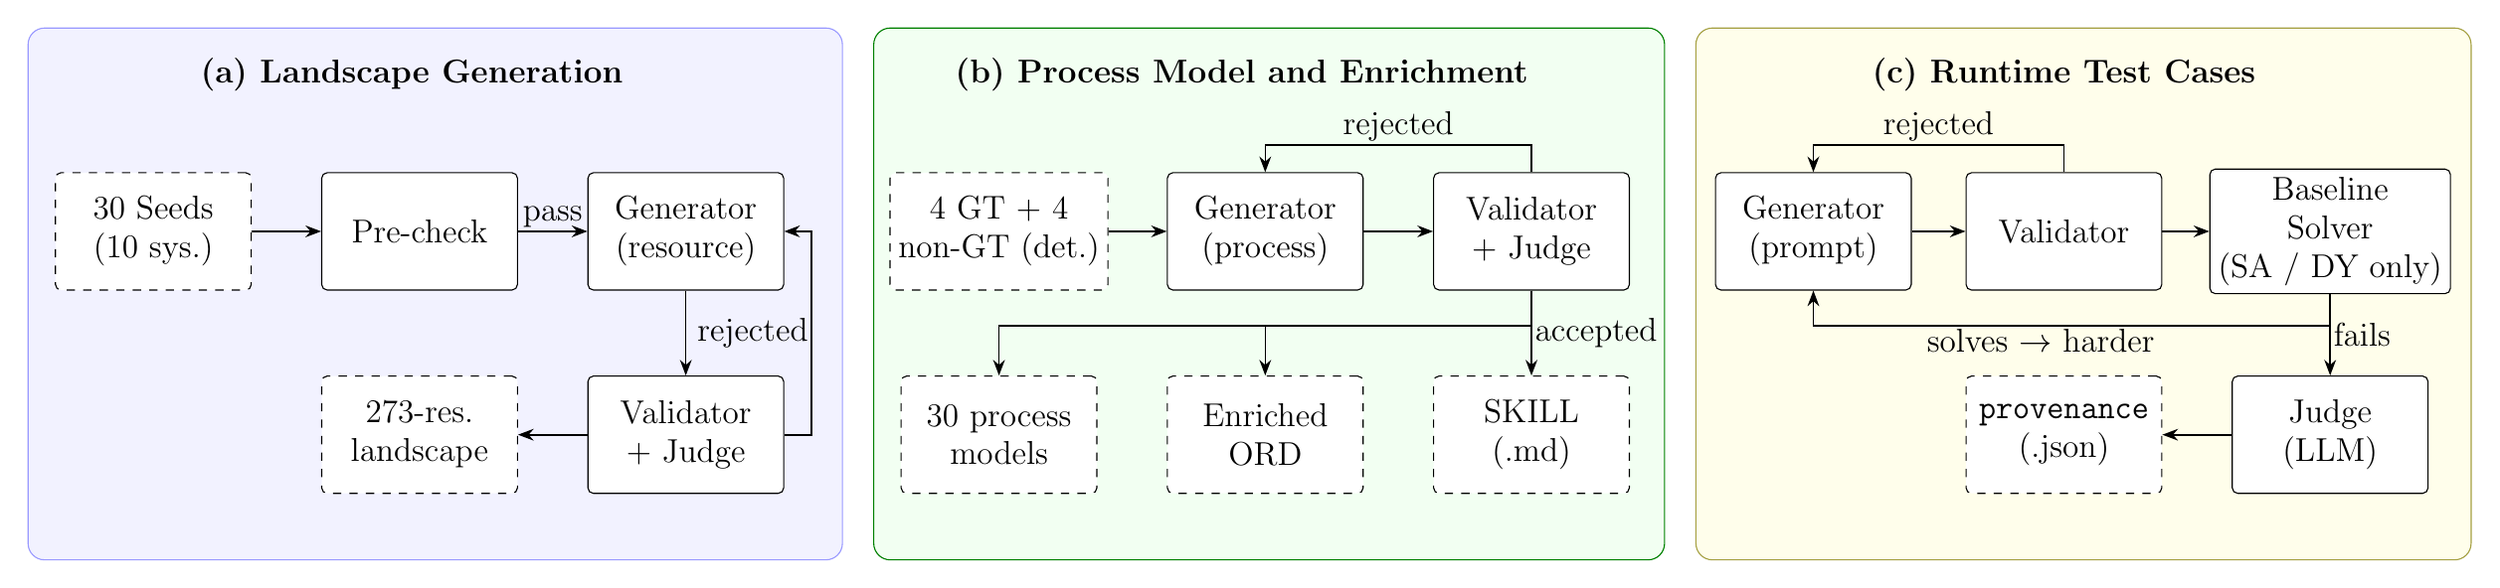
\begin{tikzpicture}[
    font=\large,
    box/.style={draw, rounded corners=2pt, minimum width=25mm, minimum height=15mm,
                align=center, inner sep=3pt, fill=white},
    io/.style={draw, dashed, rounded corners=2pt, minimum width=25mm, minimum height=15mm,
               align=center, inner sep=3pt, fill=white},
    arr/.style={-{Stealth[length=2mm]}, semithick},
    lbl/.style={font=\large, inner sep=1pt},
    ttl/.style={font=\large\bfseries}
  ]

  \begin{scope}[on background layer]
    \draw[rounded corners=6pt, fill=blue!5,   draw=blue!40]        ( -5mm, 46mm) rectangle (99mm, -22mm);
    \draw[rounded corners=6pt, fill=green!5,  draw=green!50!black] (103mm, 46mm) rectangle (204mm, -22mm);
    \draw[rounded corners=6pt, fill=yellow!8, draw=yellow!60!black](208mm, 46mm) rectangle (307mm, -22mm);
  \end{scope}

  \node[ttl] at (44mm, 40mm) {(a) Landscape Generation};
  \node[io]  (seeds)    at ( 11mm, 20mm) {30 Seeds\\(10 sys.)};
  \node[box] (precheck) at ( 45mm, 20mm) {Pre-check};
  \node[box] (genA)     at ( 79mm, 20mm) {Generator\\(resource)};
  \node[box] (gateA)    at ( 79mm,  -6mm) {Validator\\+ Judge};
  \node[io,  align=center] (landout) at ( 45mm,  -6mm) {273-res.\\landscape};
  \draw[arr] (seeds.east)    -- (precheck.west);
  \draw[arr] (precheck.east) -- node[above,lbl]{pass} (genA.west);
  \draw[arr] (genA.south)    -- (gateA.north);
  \draw[arr] (gateA.west)    -- node[above,lbl]{} (landout.east);
  \draw[arr] (gateA.east)    -- ++(3.5mm,0) |- node[left,lbl,pos=0.25]{rejected} (genA.east);

  \node[ttl] at (150mm, 40mm) {(b) Process Model and Enrichment};
  \node[io]  (sel)    at (119mm, 20mm) {4 GT + 4\\non-GT (det.)};
  \node[box] (genB)   at (153mm, 20mm) {Generator\\(process)};
  \node[box] (gateB)  at (187mm, 20mm) {Validator\\+ Judge};
  \node[io, align=center] (casesB)  at (119mm,  -6mm) {30 process\\models};
  \node[io, align=center] (enrichB) at (153mm,  -6mm) {Enriched\\ORD};
  \node[io, align=center] (skillsB) at (187mm,  -6mm) {SKILL\\(.md)};
  \draw[arr] (sel.east)   -- (genB.west);
  \draw[arr] (genB.east)  -- (gateB.west);
  \draw[arr] (gateB.north) -- ++(0,3.5mm) -| node[above,lbl,pos=0.25]{rejected} (genB.north);
  \draw[arr] (gateB.south) -- node[right,lbl,pos=0.5]{accepted} (skillsB.north);
  \draw[arr] (gateB.south) -- ++(0,-4.5mm) -| (casesB.north);
  \draw[arr] (gateB.south) -- ++(0,-4.5mm) -| (enrichB.north);

  \node[ttl] at (255mm, 40mm) {(c) Runtime Test Cases};
  \node[box] (genC)    at (223mm, 20mm) {Generator\\(prompt)};
  \node[box] (valC)    at (255mm, 20mm) {Validator};
  \node[box] (solverC) at (289mm, 20mm) {Baseline\\Solver\\(SA / DY only)};
  \node[box] (judgeC)  at (289mm,  -6mm) {Judge\\(LLM)};
  \node[io,  align=center] (provC) at (255mm,  -6mm) {\texttt{provenance}\\(.json)};
  \draw[arr] (genC.east)     -- (valC.west);
  \draw[arr] (valC.east)     -- (solverC.west);
  \draw[arr] (solverC.south) -- node[right,lbl]{fails} (judgeC.north);
  \draw[arr] (judgeC.west)   -- node[above,lbl]{} (provC.east);
  \draw[arr] (solverC.south) -- ++(0,-4mm) -|
    node[below,lbl,pos=0.28]{solves $\to$ harder} (genC.south);
  \draw[arr] (valC.north)    -- ++(0,3.5mm) -| node[above,lbl,pos=0.25]{rejected} (genC.north);
  \end{tikzpicture}}%
  \caption{Benchmark construction pipelines. (a)~Landscape: seeds, expanded via pre-check, LLM generation, and Validator/Judge gate. (b)~Process model and enrichment: one accepted model yields Enriched-ORD fields, a SKILL.md, and design-time activity cases. (c)~Runtime cases: the single-LLM baseline-solver difficulty gate applies only to the retrieval-driven modes (Skill-Adjusted, Dynamic); Skill-Guided is scored by routing alone and Out-of-Scope uses a programmatic absence check, so both bypass the gate.}
  \label{fig:pipelines}
  \end{figure*}
  
This approach is used rather than relying on embedding similarity, because ambiguity can be defined directly over interpretable ORD fields to ensure that benchmark difficulty remains transparent, reproducible, and independent of any particular embedding model. 

\textbf{Landscape generation.} With the resource model, system landscape, and ambiguity metric defined, the landscape can be populated with resources. The goal is a landscape dense enough that no retrieval method succeeds by trivial matching. The generation follows three sequential steps (Fig.~\ref{fig:pipelines}(a)): seed generation, iterative gap-filling, and quality control.

Seed generation starts from 30 LLM-generated seed resources (3 per system), with entity types assigned so that all 50 \texttt{sap.odm} types are referenced from the start. From the seeds, iterative gap-filling grows the landscape round by round, generating resources at specific similarity tiers: for each existing resource, the loop aims to surround it with a neighbourhood of at least 3 HIGH-ambiguity ($\geq$0.50), 5 MEDIUM-ambiguity (0.25--0.49), and 5 LOW-ambiguity (0.10--0.24) neighbours, generating a new resource whenever a tier is under-filled. Before each LLM call, a pre-check (Fig.~\ref{fig:pipelines}(a)) verifies that a resource with the intended properties can reach the target tier; if not, the gap is skipped.

Every generated candidate passes a two-stage quality gate: a deterministic ORD~v1.16 validator runs first at zero LLM cost (checking required fields), followed by an LLM Judge that evaluates coherence with the system domain, non-duplication, entity-type references, and a domain-sensible description. All LLM calls use \texttt{claude-haiku-4.5} at temperature 0.0 with a fixed seed. Accepted resources become seeds for subsequent rounds. A final pass removes near-textual-duplicates that the structural generation score could not detect. Appendix~\ref{appendix:landscape-audit} details the algorithm.

Generation targets 300 resources, a mid-scale size, large enough to create genuine cross-system confusion without forcing resources from entity-type categories that rarely appear across real enterprise systems.



\textbf{Process models and semantic enrichment.} After fixing the enterprise resource landscape, 30 enterprise process models (15 BPMN, 15 CMMN) are generated as controlled sources of process semantics (Fig.~\ref{fig:pipelines}(b)). Each model is constructed from a deterministically selected resource pool consisting of four resources that have reached the required neighbourhood ambiguity level and four resources that have not, while spanning at least three namespaces. The generator creates a coherent 8-activity process model grounded in this pool, assigning one activity to each selected resource.

Each generated process model passes a two-stage validation gate. First, a deterministic validator verifies structural correctness and ensures that all referenced \texttt{ordId}s exist in the resource landscape. Second, an LLM Judge evaluates whether the generated process is semantically coherent from a domain perspective. The corresponding generator and judge prompts are provided in Appendix~\ref{appendix:dt-cases}.

Only accepted process models are used for semantic enrichment. For each confirmed activity--resource pair, the generation pipeline writes four typed semantic fields, \texttt{capabilities}, \texttt{useCases}, \texttt{partOfGroups}, and \texttt{processNext}, back into the corresponding ORD document, creating the Enriched-ORD state. Figure~\ref{fig:enrichment} illustrates how process activities are mapped to ORD resources and how additional semantic context is derived without modifying resource identities or existing base fields. Furthermore, each accepted process model produces a \emph{skill artefact}: a structured markdown representation of the process steps, with each step explicitly linked to its confirmed resource \citep{anthropic_skills_2025}. This representation makes the generated process knowledge directly consumable by LLM-based agents.

To quantify the effect of this enrichment on resource distinguishability, the ambiguity metric is extended by three of the newly introduced fields (\texttt{capabilities}, \texttt{partOfGroups}, and \texttt{useCases}). Each field contributes only when both resources in a comparison pair contain the respective attribute, extending the original six-field metric (Table~\ref{tab:ambiguity-metric}) to a maximum of nine dimensions. The field \texttt{processNext} is excluded because it represents directed process relationships between resources rather than an intrinsic property of an individual resource. Comparing identical resource pairs under the original and extended metrics isolates the contribution of semantic enrichment to ambiguity reduction. The complete nine-dimension formulation and an illustrative example are provided in Appendix~\ref{appendix:disambiguation}.

\textbf{Test cases.} With the landscape and its enrichment in place, the benchmark needs concrete tasks that exercise resource selection against the graded distractors built into it. To this end it provides two case families. \emph{Design-time cases} test activity-to-resource matching: given a process step, which landscape resource realises it? Each of the 30 process models yields eight activity cases, one per resource in the pool. Ground-truth pairings are fixed by construction: the Generator assigns one resource per activity and the two-stage gate verifies the pairing is structurally valid and domain-coherent, so every label is machine-verified rather than hand-annotated. These cases make the benchmark a substrate for automating semantic enrichment: a retrieval method that can map process activities to ORD resources can populate the enrichment fields automatically, turning process models into an annotation pipeline.

\emph{Runtime cases} test resource selection under real-world intent conditions. Each case targets a resource that has reached the required neighbourhood, ensuring every ground truth has genuine HIGH-tier distractors in the full landscape. Like the landscape, each case is produced by a Generator–Judge pipeline (Fig.~\ref{fig:pipelines}(c)): a Generator produces a natural-language request targeting a specific resource, and the Judge verifies the request is unambiguous and domain-coherent. Three orchestration modes reflect the degree to which a prior process definition is available, covering the enterprise spectrum from fully-guided skill execution to open-ended retrieval: \emph{Skill-Guided} (30 test cases) where a matching skill covers the full request; \emph{Skill-Adjusted} (20 test cases) where a skill applies but has gap steps that require retrieval; and \emph{Dynamic} (40 test cases) where no skill matches and the agent must select from the full landscape. An Out-of-Scope condition (20 test cases) tests abstention when no resource can satisfy the request. 

For the retrieval-driven modes, a Baseline-Solver gate additionally discards any case a trivial single-call LLM solver already solves, certifying that retained cases require structured retrieval; Skill-Guided and Out-of-Scope bypass this gate by construction. The test cases themselves are fixed; every case can run on both the Clean-ORD and Enriched-ORD landscape states, so the enrichment effect is measurable as a controlled variable without changing the request or the ground truth. Appendix~\ref{appendix:rt-cases} gives the per-mode generator prompts and a solver-gate provenance trace.

\begin{figure*}[t]
  \centering
  \resizebox{0.92\textwidth}{!}{%
  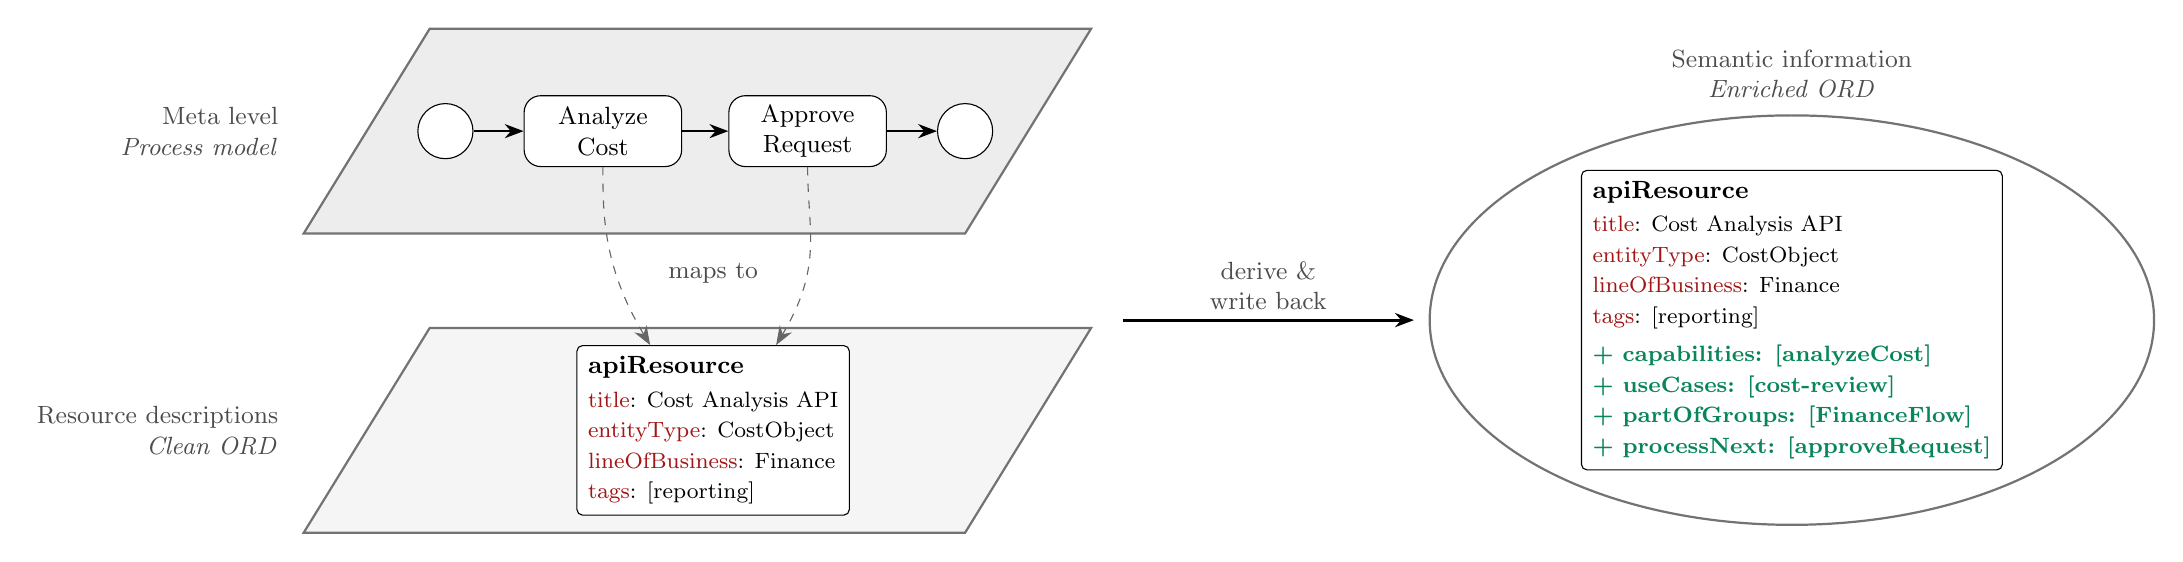
\begin{tikzpicture}[
    plane/.style={draw=black!55, thick},
    res/.style={draw, rounded corners=2pt, align=left, inner sep=4pt, fill=white,
                font=\small},
    act/.style={draw, rounded corners=6pt, minimum width=20mm, minimum height=9mm,
                align=center, inner sep=2pt, fill=white, font=\small},
    ev/.style={draw, circle, minimum size=7mm, inner sep=0pt, fill=white, font=\scriptsize},
    arr/.style={-{Stealth[length=2.4mm]}, semithick},
    maparr/.style={-{Stealth[length=2.4mm]}, dashed, black!60},
    lbl/.style={font=\small, black!70}
  ]

  % ===== Meta level: process model (upper-left plane) =====
  \fill[black!7]  (6mm,44mm) -- (90mm,44mm) -- (106mm,70mm) -- (22mm,70mm) -- cycle;
  \draw[plane]    (6mm,44mm) -- (90mm,44mm) -- (106mm,70mm) -- (22mm,70mm) -- cycle;
  \node[lbl, anchor=east, align=right] at (4mm, 57mm) {Meta level\\\textit{Process model}};
  \node[ev]  (start) at (24mm, 57mm) {};
  \node[act] (a1)    at (44mm, 57mm) {Analyze\\Cost};
  \node[act] (a2)    at (70mm, 57mm) {Approve\\Request};
  \node[ev]  (end)   at (90mm, 57mm) {};
  \draw[arr] (start) -- (a1);
  \draw[arr] (a1) -- (a2);
  \draw[arr] (a2) -- (end);

  % ===== Description layer: Clean ORD (lower-left plane) =====
  \fill[black!4]  (6mm,6mm) -- (90mm,6mm) -- (106mm,32mm) -- (22mm,32mm) -- cycle;
  \draw[plane]    (6mm,6mm) -- (90mm,6mm) -- (106mm,32mm) -- (22mm,32mm) -- cycle;
  \node[lbl, anchor=east, align=right] at (4mm, 19mm) {Resource descriptions\\\textit{Clean ORD}};
  \node[res] (clean) at (58mm, 19mm) {%
    \textbf{\small apiResource}\\[1pt]
    {\footnotesize\textcolor{jsonkey}{title}: Cost Analysis API}\\
    {\footnotesize\textcolor{jsonkey}{entityType}: CostObject}\\
    {\footnotesize\textcolor{jsonkey}{lineOfBusiness}: Finance}\\
    {\footnotesize\textcolor{jsonkey}{tags}: [reporting]}%
  };
  \draw[maparr] (a1.south) .. controls +(0,-6mm) and +(-6mm,10mm) .. ([xshift=-8mm]clean.north);
  \draw[maparr] (a2.south) .. controls +(0,-8mm) and +(6mm,10mm)  .. ([xshift=8mm]clean.north);
  \node[lbl, fill=white, inner sep=1pt] at (58mm, 39mm) {maps to};

  % ===== Semantic layer: Enriched ORD (right, in oval) =====
  \node[res, anchor=center] (enr) at (195mm, 33mm) {%
    \textbf{\small apiResource}\\[1pt]
    {\footnotesize\textcolor{jsonkey}{title}: Cost Analysis API}\\
    {\footnotesize\textcolor{jsonkey}{entityType}: CostObject}\\
    {\footnotesize\textcolor{jsonkey}{lineOfBusiness}: Finance}\\
    {\footnotesize\textcolor{jsonkey}{tags}: [reporting]}\\[3pt]
    {\footnotesize\bfseries\color{jsonnumber}+ capabilities: [analyzeCost]}\\
    {\footnotesize\bfseries\color{jsonnumber}+ useCases: [cost-review]}\\
    {\footnotesize\bfseries\color{jsonnumber}+ partOfGroups: [FinanceFlow]}\\
    {\footnotesize\bfseries\color{jsonnumber}+ processNext: [approveRequest]}%
  };
  \begin{scope}[on background layer]
    \draw[plane] (enr.center) ellipse (46mm and 26mm);
  \end{scope}
  \node[lbl, anchor=south, align=center] at (195mm, 60mm) {Semantic information\\\textit{Enriched ORD}};
  \draw[arr, line width=1pt] (110mm, 33mm) -- (147mm, 33mm)
    node[midway, above, lbl, align=center] {derive \&\\write back};
  \end{tikzpicture}}%
  \caption{Process-driven semantic enrichment of ORD. A process model is mapped onto a Clean-ORD resource; the mapping deterministically derives four typed fields (\texttt{capabilities}, \texttt{useCases}, \texttt{partOfGroups}, \texttt{processNext}) written back into the resource, yielding its Enriched-ORD state. The resource identity is preserved.}
  \label{fig:enrichment}
\end{figure*}




% ─────────────────────────────────────────────────────────────────────────────
\section{Results}
\label{sec:results}
% ─────────────────────────────────────────────────────────────────────────────



This section reports the artefacts produced by applying the methodology of Sec.~\ref{sec:design}. The resource landscape is presented first, followed by the test-case suite derived on top of it. Finally, an ambiguity analysis compares resource ambiguity under clean and semantically enriched description.



\begin{figure}[t]
  \centering
  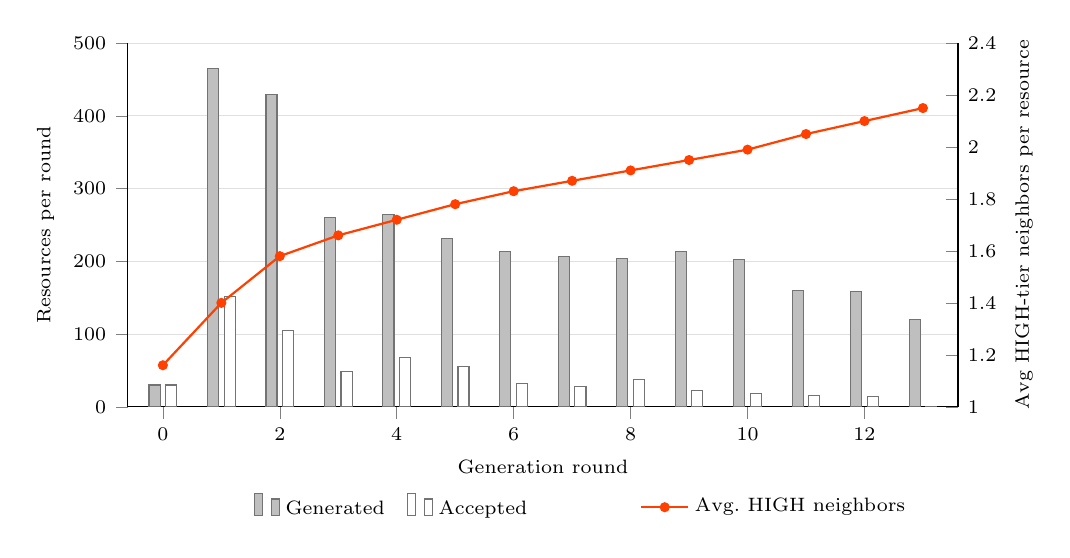
\begin{tikzpicture}
    \begin{axis}[
      width=\columnwidth, height=6.2cm,
      ybar, bar width=4pt,
      xmin=-0.6, xmax=13.6,
      xtick={0,2,4,6,8,10,12}, xticklabel style={font=\scriptsize},
      xlabel={Generation round}, xlabel style={font=\scriptsize},
      ymin=0, ymax=500,
      ytick={0,100,200,300,400,500}, yticklabel style={font=\scriptsize},
      ylabel={Resources per round}, ylabel style={font=\scriptsize},
      ymajorgrids, grid style={draw=black!12},
      axis y line*=left, axis x line*=bottom,
      tick align=outside,
      legend style={
        at={(0.32,-0.22)}, anchor=north, legend columns=2,
        draw=none, font=\scriptsize, /tikz/every even column/.append style={column sep=6pt}
      },
      legend cell align=left,
    ]
      \addplot+[fill=black!25, draw=black!55, bar shift=-3pt] coordinates
        {(0,30) (1,465) (2,430) (3,260) (4,265) (5,232) (6,213) (7,207) (8,204) (9,214) (10,202) (11,160) (12,158) (13,120)};
      \addlegendentry{Generated}
      \addplot+[fill=white, draw=black!55, bar shift=3pt] coordinates
        {(0,30) (1,152) (2,105) (3,48) (4,68) (5,55) (6,32) (7,28) (8,38) (9,22) (10,18) (11,15) (12,14) (13,1)};
      \addlegendentry{Accepted};
    \end{axis}
    \begin{axis}[
      width=\columnwidth, height=6.2cm,
      xmin=-0.6, xmax=13.6,
      xtick=\empty,
      ymin=1.0, ymax=2.4,
      ytick={1.0,1.2,1.4,1.6,1.8,2.0,2.2,2.4}, yticklabel style={font=\scriptsize},
      ylabel={Avg HIGH-tier neighbors per resource}, ylabel style={font=\scriptsize},
      axis y line*=right, axis x line=none,
      legend style={
        at={(0.78,-0.22)}, anchor=north, draw=none, font=\scriptsize
      },
      legend cell align=left,
    ]
      \addplot+[color=red!50!orange, mark=*, mark size=1.4pt, thick,
               mark options={fill=red!50!orange, draw=red!50!orange}]
        coordinates
        {(0,1.16) (1,1.40) (2,1.58) (3,1.66) (4,1.72) (5,1.78) (6,1.83) (7,1.87) (8,1.91) (9,1.95) (10,1.99) (11,2.05) (12,2.10) (13,2.15)};
      \addlegendentry{Avg.\ HIGH neighbors};
    \end{axis}
  \end{tikzpicture}
  \caption{Iterative generation convergence. Bars: candidates generated (grey) and accepted (white) per round. Circles: avg.\ HIGH-tier neighbours (sim\,$\geq$\,0.50) under the generation-time similarity (no TF-IDF text, for speed).}
  \label{fig:convergence}
\end{figure}

% --- R1: Resource Landscape (contributions 1+2) ---
\textbf{Resource Landscape.} The generation loop began at round~0 with 30 seed resources (3 per system) and ran for 13 further rounds (Fig.~\ref{fig:convergence}). Acceptances fell steadily as the landscape filled: round~1 accepted 152 of 465 candidates, round~3 only 48, and by round~13 just one candidate passed the gate. The falling acceptance count and the flattening HIGH-tier curve are two views of the same saturation, as more resources were placed, new candidates had to be similar enough to fill remaining neighbourhood gaps yet distinct enough to clear the quality gate, a window that narrowed with every round. The average HIGH-tier neighbourhood accordingly rose steeply at first (1.16 at round~0 to 1.72 by round~4) and then flattened towards 2.15, since each newly added resource contributed fewer novel HIGH-tier pairings once the dense regions were already covered. 

Generation stopped at the 300-resource target. By that point acceptances had collapsed to one per round, so the loop had naturally saturated. A final near-duplicate pass recomputed full similarity on the fixed 300-resource corpus, including the TF-IDF text score omitted during generation for speed, and removed 27 near-duplicate pairs, leaving 273 resources.



The quality gate filtered most generated candidates. Of those that reached the LLM Judge, 2{,}936 were rejected. The most common reasons (which can overlap for a single candidate) were domain incoherence (2{,}363 cases, for example an IT-service-management ticket proposed inside an ERP finance system), unjustified entity-type references (1{,}720), and duplication of an existing resource (1{,}393). A further 85 were discarded by the pre-check before any LLM call. An example rejection log entry is in Appendix~\ref{appendix:landscape-audit}.

The resulting landscape (Table~\ref{tab:landscape-systems}) spans ten systems whose resources cluster around shared ODM entity types, producing the confusable cross-system neighbourhoods the benchmark targets. Appendix~\ref{appendix:landscape-results} provides a graph visualisation that makes this cross-system similarity visible. 

Recomputed on the final 273-resource corpus under the full similarity metric (including the TF-IDF text score), each resource carried on average 1.74 HIGH-tier, 11.0 MEDIUM-tier, and 49.8 LOW-tier neighbours; this figure is lower than the 2.15 reported during generation (Fig.~\ref{fig:convergence}), because the full metric is stricter than the fast generation-time score and the near-duplicate pass removed 27 resources. Exactly 70 of the 273 resources reached the required neighbourhood defined in Sec.~\ref{sec:design} (HIGH$\geq$3, MEDIUM$\geq$5, LOW$\geq$5), forming the ground-truth-eligible set used as targets for retrieval test cases. The resource-type distribution (50\% \texttt{apiResource}, 24\% \texttt{agent}, 26\% \texttt{dataProduct}) mirrors real enterprise landscapes. The 70 eligible resources were not distributed uniformly: \texttt{sap.ehs} and \texttt{sap.sf} contributed fewer because their entity types (safety incidents, HR objects) are less cross-domain than those of \texttt{corp.itsm} or \texttt{my.mes}, which share business objects (Vendor, Material) with several systems.


\begin{table}[!t]
  \small\centering\footnotesize
  \caption{ORD-Bench landscape: 10 namespaces, 273 resources. GT = resources that satisfy the required neighbourhood (HIGH$\geq$3, MEDIUM$\geq$5, LOW$\geq$5).}
  \label{tab:landscape-systems}
  \begin{tabularx}{\linewidth}{@{} l l >{\centering\arraybackslash}X >{\centering\arraybackslash}X >{\centering\arraybackslash}X >{\centering\arraybackslash}X >{\centering\arraybackslash}X @{}}
  \toprule
  \textbf{Namespace} & \textbf{Domain} & \textbf{API} & \textbf{Agt} & \textbf{DP} & \textbf{Tot} & \textbf{GT} \\
  \midrule
  \texttt{sap.s4}       & ERP, Finance     & 14 & 6 & 8  & 28 & 10 \\
  \texttt{sap.sf}       & HR               & 15 & 6 & 5  & 26 &  4 \\
  \texttt{sap.ariba}    & Procurement      & 13 & 3 & 7  & 23 &  7 \\
  \texttt{sap.crm}      & Sales, Customer  & 11 & 7 & 9  & 27 &  7 \\
  \texttt{sap.ehs}      & Safety, Env.     & 15 & 6 & 9  & 30 &  4 \\
  \texttt{corp.itsm}    & IT Service Mgmt  & 14 & 8 & 7  & 29 &  9 \\
  \texttt{my.mes}       & Mfg. Execution   & 15 & 5 & 9  & 29 &  9 \\
  \texttt{workday.hcm}  & HR (non-SAP)     & 13 & 9 & 4  & 26 &  6 \\
  \texttt{emarsys.cx}   & Marketing, CX    & 13 & 8 & 8  & 29 &  8 \\
  \texttt{siemens.plm}  & Prod. Lifecycle  & 14 & 8 & 4  & 26 &  6 \\
  \midrule
  \textbf{Total}        &                  & \textbf{137} & \textbf{66} & \textbf{70} & \textbf{273} & \textbf{70} \\
  \bottomrule
  \end{tabularx}
\end{table}


% --- R2: Semantic Enrichment (contribution 3) ---
\begin{figure}[t]
  \centering
  
\includegraphics[width=0.82\columnwidth]{figures/fig_scatter.pdf}
  \caption{Disambiguation effect of the semantic enrichment. Each point is one of the 2\,415 pairs among the 70 enriched resources: six-field ambiguity (x) versus extended nine-dimension ambiguity (y). All 85 HIGH-tier pairs ($\geq$0.50, dark) drop below the diagonal, and drop most where original ambiguity was highest. Low-ambiguity pairs (light) mostly stay near the diagonal; a minority rise slightly. Overall, 2\,176 of the 2\,415 pairs move apart.}
  \label{fig:disambiguation}
\end{figure}

% Superseded by the scatter above; bar chart kept for reference.
% \begin{figure}[t]
%   \centering
%   \begin{tikzpicture}
%     \begin{axis}[
%       width=\columnwidth, height=5.6cm,
%       ybar, bar width=15pt,
%       symbolic x coords={all, high},
%       xtick=data,
%       enlarge x limits=0.5,
%       xticklabels={All enriched pairs\\($n{=}2415$), Previously HIGH pairs\\($n{=}85$)},
%       xticklabel style={font=\scriptsize, align=center},
%       ymin=0, ymax=0.72,
%       ytick={0,0.1,...,0.7}, yticklabel style={font=\scriptsize},
%       ylabel={Mean pairwise ambiguity}, ylabel style={font=\scriptsize},
%       ymajorgrids, grid style={draw=black!12},
%       axis y line*=left, axis x line*=bottom,
%       tick align=outside,
%       nodes near coords, nodes near coords style={font=\tiny},
%       nodes near coords={\pgfmathprintnumber[fixed, precision=3]{\pgfplotspointmeta}},
%       every node near coord/.append style={yshift=1pt},
%       legend style={
%         at={(0.5,-0.22)}, anchor=north, legend columns=2,
%         draw=none, font=\scriptsize, /tikz/every even column/.append style={column sep=8pt}
%       },
%       legend cell align=left,
%     ]
%       \addplot+[fill=black!25, draw=black!55, bar shift=-8pt] coordinates
%         {(all,0.111) (high,0.643)};
%       \addlegendentry{Six-field metric}
%       \addplot+[fill=white, draw=black!55, bar shift=8pt] coordinates
%         {(all,0.084) (high,0.461)};
%       \addlegendentry{Extended metric ($+$ semantic)};
%     \end{axis}
%   \end{tikzpicture}
%   \caption{Disambiguation effect of the semantic layer. Mean pairwise ambiguity under the six-field metric (grey) versus the extended nine-dimension metric (white). Left: all 2\,415 pairs where both resources carry the semantic fields. Right: the 85 pairs that were HIGH-tier under the six-field metric.}
%   \label{fig:disambiguation}
% \end{figure}

\textbf{Semantic Enrichment.} The semantic enrichment is derived from generated enterprise process models. Of 57 process-model generation attempts, 30 were accepted (8 rejected by the deterministic validator, 16 by the LLM Judge, and 3 abandoned after the retry budget). Each accepted model uses four resources that have reached the required ambiguity neighbourhood and four that have not. Only the former receive the four process-derived semantic fields; the supporting resources stay at Clean-ORD level. Enrichment is therefore targeted at the 70 confusable resources rather than landscape-wide; Appendix~\ref{appendix:landscape-example} shows a representative resource in its Clean-ORD and Enriched-ORD state.

To test whether this semantic enrichment improves distinguishability between resources, the six-field and the extended ambiguity metric are compared on the same resource pairs. Figure~\ref{fig:disambiguation} shows the effect across all 2{,}415 pairs. Across all $\binom{70}{2}{=}2{,}415$ pairs, the mean pairwise ambiguity dropped from 0.111 to 0.084 ($-24.5\%$). Looking only at the 85 pairs whose six-field score exceeded the HIGH threshold ($\geq$0.50), the ones that actually risk confusion, the mean dropped from 0.643 to 0.461 ($-28.3\%$).

Enrichment lowered structural ambiguity most where the risk of confusion was highest. The effect is also visible at the resource level: 52 of the 273 resources shed at least one HIGH-tier neighbour under the extended metric while none gained one, dissolving 128 HIGH-tier pairings in total. Enrichment therefore does not merely shift averages but pulls confusable resources apart into distinguishable ones. An embedding-based view of the same enrichment, which moves in the opposite direction, is analysed in Sec.~\ref{sec:discussion}.

% --- R3: Test-Case Suite (contribution 4) ---
\textbf{Test-Case Suite.} On top of the landscape the benchmark ships 350 test cases as a reusable substrate, split into a \emph{design-time set} and a \emph{runtime set}. The design-time set reuses the 30 accepted process models: each contributes eight activity cases, giving 240 design-time cases with four activities drawn from resources that had reached the required neighbourhood and four from those that had not.

The \emph{runtime set} spans four modes, each with its own acceptance criterion. The two retrieval-driven modes, Skill-Adjusted and Dynamic, were built under a Baseline-Solver gate that regenerated a case until a trivial single-call solver could no longer answer it: across their 60 cases this took 118 generation iterations, 37 rejected as too easy and regenerated with more implicit phrasing, and a further 25 rejected by the Judge for realism or naming violations. Skill-Guided (30 cases) is scored by routing accuracy rather than retrieval difficulty, so it bypasses the solver gate; all 30 were accepted on the first attempt. Out-of-Scope (20 cases) has no ground-truth resource, so instead of the solver gate an absence check discards any request that lies too close to an existing resource; this rejected 9 of the 29 generated candidates. Together the four modes yield 110 runtime cases, bringing the benchmark to 350 test cases.

To confirm that difficulty was stable rather than an artefact of a single generation-time solver run, the 90 retrieval-driven runtime cases were re-certified by running the baseline solver five independent times per case and flagging any case it solved. Under the strict criterion (solved in zero of five runs), 91.1\% of cases (82/90) certified as robust, with a mean difficulty of 0.94; per mode, Skill-Guided certified 30/30, Skill-Adjusted 18/20, and Dynamic 34/40, with the six residual cases solved on only a minority of runs. Difficulty was therefore a reproducible property of the cases rather than a single-run coincidence.


\begin{table*}[t]
  \centering\footnotesize
  \renewcommand{\arraystretch}{1.2}
  \setlength{\tabcolsep}{5pt}
  \caption{One test case per family. DT = design-time, SG = Skill-Guided, SA = Skill-Adjusted, DY = Dynamic, OOS = Out-of-Scope.}
  \label{tab:example-cases}
  \begin{tabularx}{\textwidth}{@{} l c >{\raggedright\arraybackslash}X >{\raggedright\arraybackslash\ttfamily\scriptsize}p{0.28\textwidth} @{}}
  \toprule
  \textbf{Family} & \textbf{\emph{n}} & \textbf{Example request / step label} & \normalfont\textbf{Ground-truth target} \\
  \midrule
  \textbf{DT} & 240 & \emph{``Request Production Schedule Adjustment --- initiate a change request to modify production orders based on demand forecasting or supply constraints.''} & sap.crm:apiResource:\allowbreak MachineProductionOrderIntegration \\
  \midrule
  \textbf{SG} & 30 & \emph{``We need to handle a product engineering change end to end --- from assessing production impact through validating materials are compliant with the new design.''} & \normalfont Routes to skill proc\_022 (4 confirmed steps) \\
  \textbf{SA} & 20 & \emph{``Establish a procurement and delivery workflow coordinating vendor assessment and enriched customer purchases, including handling customer grievances and reconciling disagreements.''} & \normalfont proc\_033 + gaps: CustomerOrder\-FulfillmentTracking, CustomerAccount\-DisputeManagement \\
  \textbf{DY} & 40 & \emph{``Pull up a recent issue a customer reported last week so I can see what we promised and whether we're on track.''} & corp.itsm:apiResource:\allowbreak ServiceTicketOrderManagementAPI \\
  \midrule
  \textbf{OOS} & 20 & \emph{``Automatically flag suppliers whose credit ratings deteriorated in the past 90 days so we can reduce order volumes before a cash-flow problem.''} & \normalfont None --- correct action is refusal \\
  \bottomrule
  \end{tabularx}
\end{table*}

Table~\ref{tab:example-cases} shows one accepted case per family. Design-time cases were terse activity labels resolved against the in-model resource pool; runtime cases were full natural-language requests resolved against the whole landscape. Each mode added a distinct source of difficulty: typed distractors, implied gap steps, cross-namespace confusables, or a genuinely absent capability. How retrieval methods perform on these cases is the subject of a companion paper.




% ─────────────────────────────────────────────────────────────────────────────
\section{Discussion}
\label{sec:discussion}
% ─────────────────────────────────────────────────────────────────────────────

This section first interprets the results with respect to the research question, before discussing the limitations of the work and directions for future research.

\textbf{Interpretation of findings.} The benchmark fills a specific gap: its difficulty is a controlled property of semantic ambiguity between typed enterprise resources, not a by-product of catalogue size. Three properties make its results transparent and traceable: (1)~the auditable ambiguity metric assigns every pair a tier that can be traced back to the six ORD fields; (2)~the adversarial difficulty gate removes trivial test cases, so measured accuracies reflect genuine selection ability rather than easy wins; (3)~the clean and enriched description states isolate the semantic enrichment $\Delta$ as an independent factor, so an observed gain is attributable to the semantic fields and not to case-difficulty drift. The five-run difficulty certification (91.1\% of retrieval-driven cases robust) confirms that these properties hold in practice: the benchmark is not merely designed to be hard, but demonstrably is.


\begin{figure}[t]
  \centering
  \definecolor{embHIGH}{HTML}{1C5CAB}
  \definecolor{embMED}{HTML}{2A78D6}
  \definecolor{embLOW}{HTML}{5598E7}
  \definecolor{embNONE}{HTML}{86B6EF}
  \begin{tikzpicture}
    \begin{axis}[
      width=\columnwidth, height=5.8cm,
      boxplot/draw direction=y,
      xtick={1,2,3,4},
      xticklabels={HIGH\\{\tiny$\geq$0.50}\\{\tiny$n{=}237$},
                   MEDIUM\\{\tiny .25--.49}\\{\tiny$n{=}1499$},
                   LOW\\{\tiny .10--.24}\\{\tiny$n{=}6801$},
                   NONE\\{\tiny$<$.10}\\{\tiny$n{=}28591$}},
      xticklabel style={font=\scriptsize, align=center},
      ymin=0, ymax=1.02,
      ytick={0,0.2,0.4,0.6,0.8,1.0}, yticklabel style={font=\scriptsize},
      ylabel={Embedding cosine}, ylabel style={font=\scriptsize},
      ymajorgrids, grid style={draw=black!12},
      axis y line*=left, axis x line*=bottom, tick align=outside,
    ]
      \addplot+[boxplot prepared={lower whisker=0.443, lower quartile=0.657, median=0.737,
        upper quartile=0.811, upper whisker=0.916, draw position=1, box extend=0.5},
        solid, fill=embHIGH, fill opacity=0.9, draw=black!55, line width=0.6pt,
        boxplot/every median/.style={white, line width=1.2pt}] coordinates {};
      \node[font=\tiny\bfseries, white, anchor=south] at (axis cs:1,0.737) {0.74};
      \addplot+[boxplot prepared={lower whisker=0.268, lower quartile=0.500, median=0.599,
        upper quartile=0.681, upper whisker=0.927, draw position=2, box extend=0.5},
        solid, fill=embMED, fill opacity=0.9, draw=black!55, line width=0.6pt,
        boxplot/every median/.style={white, line width=1.2pt}] coordinates {};
      \node[font=\tiny\bfseries, white, anchor=south] at (axis cs:2,0.599) {0.60};
      \addplot+[boxplot prepared={lower whisker=0.222, lower quartile=0.411, median=0.475,
        upper quartile=0.538, upper whisker=0.728, draw position=3, box extend=0.5},
        solid, fill=embLOW, fill opacity=0.9, draw=black!55, line width=0.6pt,
        boxplot/every median/.style={white, line width=1.2pt}] coordinates {};
      \node[font=\tiny\bfseries, white, anchor=south] at (axis cs:3,0.475) {0.48};
      \addplot+[boxplot prepared={lower whisker=0.108, lower quartile=0.289, median=0.346,
        upper quartile=0.410, upper whisker=0.593, draw position=4, box extend=0.5},
        solid, fill=embNONE, fill opacity=0.9, draw=black!55, line width=0.6pt,
        boxplot/every median/.style={white, line width=1.2pt}] coordinates {};
      \node[font=\tiny\bfseries, white, anchor=south] at (axis cs:4,0.346) {0.35};
    \end{axis}
  \end{tikzpicture}
  \caption{Embedding cosine grouped by structural tier (37\,128 pairs). Median cosine rises monotonically with the tier (NONE $\to$ HIGH), confirming the field-based metric captures a real difficulty signal independent of embeddings ($r{=}0.63$ with structural score).}
  \label{fig:embedding-validation}
\end{figure}

\textbf{Field-based versus embedding difficulty.} Scoring difficulty from typed fields rather than embeddings serves two purposes: it keeps every tier assignment auditable, and it avoids handing embedding-based retrievers a difficulty structure defined in their own representation, which keeps the benchmark fair across retrieval families. 


Furthermore, the metric captures a real difficulty signal rather than an arbitrary construct. This is confirmed by two findings: First, the field-based tiers and an independent embedding model (\texttt{text-embedding-3-large}) \emph{agree} on which pairs are confusable: their scores correlate at $r=0.63$, and median embedding cosine rises monotonically with the structural tier, from 0.35 for unrelated pairs to 0.74 for HIGH-tier pairs (Fig.~\ref{fig:embedding-validation}). The structural metric is therefore not an arbitrary construct; it captures a difficulty signal a completely different representation also sees. Second, a PCA projection of the same embeddings (Appendix~\ref{appendix:landscape-results}) shows the ten namespaces fully intermixed while resource types form distinct regions, as resources group by what they do, not by which system they belong to, matching the metric's cross-type penalty. At the same time the agreement is only partial ($r=0.63$, not 1.0), and this gap is intentional: the metric adds a cross-type penalty and a cross-namespace bonus that raw embedding cosine does not have. Benchmark difficulty is thus deliberately \emph{not} a copy of what an embedding retriever measures.


\textbf{Influence of semantic enrichment.} Comparing the same resources under clean and enriched descriptions produces the paper's sharpest lesson. Writing the process-derived semantic fields back into a resource moves the two similarity measures in \emph{opposite} directions on the very same pairs. The structural metric drops by up to $28.3\%$ on the most confusable pairs (Fig.~\ref{fig:disambiguation}), whereas embedding cosine \emph{rises}: with the clean text embedding \texttt{title}, \texttt{shortDescription} and \texttt{description}, and the enriched text appending the four semantic fields, the mean cosine across all 2{,}415 both-enriched pairs climbs from 0.392 to 0.501 ($+27.7\%$), and it rises even for mixed pairs where only one resource is enriched (Fig.~\ref{fig:disambiguation-embedding}).

This is not a contradiction but a statement about representation. A method that reads the typed fields as discrete signals (namespace, entity-type, capability filters) sees two resources with disjoint capabilities pushed apart and disambiguates better; a method that compresses every field into one vector sees the added topical text pull the vectors together and disambiguates worse. Enrichment thus helps only when the retrieval mechanism and the enriched field types are structurally aligned. A benchmark that fixed a single description state could not expose this dependency at all, which is precisely why ORD-Bench ships both states.

\begin{figure}[t]
  \centering
  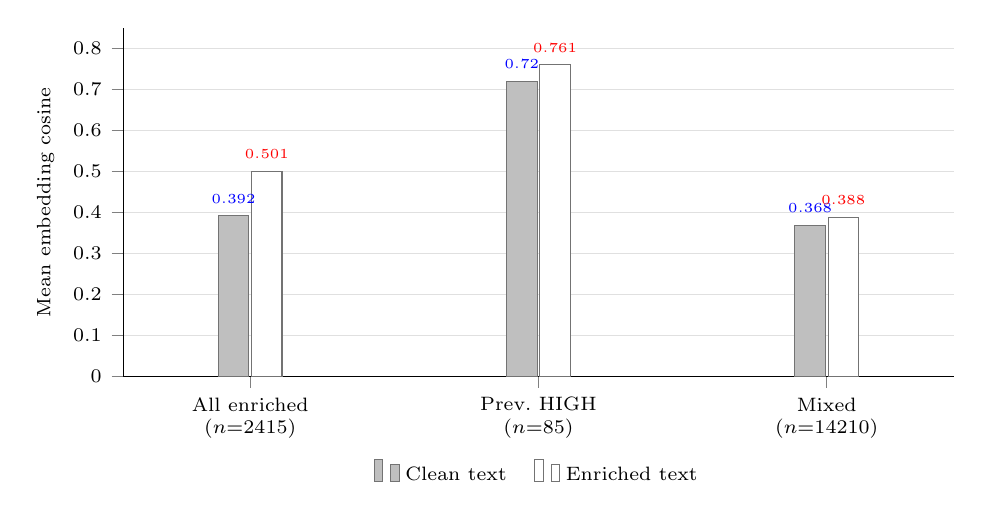
\begin{tikzpicture}
    \begin{axis}[
      width=\columnwidth, height=6.0cm,
      ybar, bar width=11pt,
      symbolic x coords={all, high, mixed},
      xtick=data,
      enlarge x limits=0.22,
      xticklabels={All enriched\\($n{=}2415$), Prev.\ HIGH\\($n{=}85$), Mixed\\($n{=}14210$)},
      xticklabel style={font=\scriptsize, align=center},
      ymin=0, ymax=0.85,
      ytick={0,0.1,...,0.8}, yticklabel style={font=\scriptsize},
      ylabel={Mean embedding cosine}, ylabel style={font=\scriptsize},
      ymajorgrids, grid style={draw=black!12},
      axis y line*=left, axis x line*=bottom,
      tick align=outside,
      nodes near coords, nodes near coords style={font=\tiny},
      nodes near coords={\pgfmathprintnumber[fixed, precision=3]{\pgfplotspointmeta}},
      every node near coord/.append style={yshift=1pt},
      legend style={
        at={(0.5,-0.22)}, anchor=north, legend columns=2,
        draw=none, font=\scriptsize, /tikz/every even column/.append style={column sep=8pt}
      },
      legend cell align=left,
    ]
      \addplot+[fill=black!25, draw=black!55, bar shift=-6pt] coordinates
        {(all,0.392) (high,0.720) (mixed,0.368)};
      \addlegendentry{Clean text}
      \addplot+[fill=white, draw=black!55, bar shift=6pt] coordinates
        {(all,0.501) (high,0.761) (mixed,0.388)};
      \addlegendentry{Enriched text};
    \end{axis}
  \end{tikzpicture}
  \caption{Embedding cosine on the same pairs, clean text (grey) versus enriched text (white). Unlike the structural metric in Fig.~\ref{fig:disambiguation}, embedding cosine \emph{rises} in every group once semantic text is added. The mixed group ($n{=}14\,210$) covers pairs where only one resource is enriched.}
  \label{fig:disambiguation-embedding}
\end{figure}

\textbf{Asymmetric enrichment.} One design choice affects how the enrichment results should be read: the Enriched-ORD state writes semantic fields only into the 70 highly ambiguous resources, not into the 203 non-eligible distractors. For methods reading typed fields, this asymmetry is intentional: it widens the distinctive gap between the target resource and its competitors, exactly what the enrichment $\Delta$ measures. For embedding-based retrieval it can work in the opposite direction: the target resource's vector shifts into a richer topical region while un-enriched neighbours stay put, which in some configurations reduces cosine distance to resources in adjacent topics. The mixed-pair experiment ($n{=}14{,}210$ pairs where only one resource is enriched) directly tests this: mean embedding cosine rises there too, from 0.368 to 0.388 ($+5.3\%$), with 10{,}517 of the 14{,}210 pairs becoming more similar, confirming the vector-blurring mechanism is not an artefact of the 70-resource asymmetry but a property of how embeddings respond to added context regardless of which side of the pair is enriched.

\textbf{Limitations.} A first group of limitations concerns the ambiguity metric itself. Equal weights across the six dimensions are a deliberate, auditable default, since differential weights would require a labelled confusion dataset that does not exist for ORD resources. A sensitivity analysis varying the weights is the natural next step, and the enrichment effect is only robust if it persists under plausible re-weightings. A related caveat concerns the embedding-cosine result: enrichment adds typed fields but leaves the base free-text descriptions (\texttt{description}, \texttt{shortDescription}) unchanged, so the observed rise in cosine may partly reflect appended structured tokens rather than genuine semantic convergence. Fairly evaluating embedding methods under \emph{full} enrichment would require rewriting the free-text descriptions too, which the current design holds fixed to keep the two states comparable.

A second group concerns test case ground truth and difficulty. Ground truth is fixed by construction and machine-verified (deterministic validator plus LLM Judge) rather than confirmed by independent human annotators, and no held-out partition was constructed. Both a human-validated gold set and a held-out split are future priorities. Difficulty was certified over five solver runs, but the solver is not fully deterministic, so a few cases were solved on only one or two runs and sit close to the difficulty cut-off; more runs would place them more reliably.

The suite is also intentionally modest in size: 350 cases split into a design-time set and four runtime families (Skill-Guided, Skill-Adjusted, Dynamic, Out-of-Scope). Because the cases are adversarially constructed rather than randomly sampled, the design prioritises \emph{systematic coverage} of the retrieval scenarios over statistical representativeness: each family targets a distinct selection challenge (typed distractors, implied gap steps, cross-namespace confusables, and genuinely absent capabilities), and each case is a purpose-built ambiguity configuration surrounded by graded distractors. The benchmark therefore emphasises representative coverage of enterprise selection scenarios rather than sample size. A consequence is that per-family case counts are small, so any downstream evaluation on individual families should report results as directional rather than as statistically powered estimates; scaling each family while preserving its controlled construction is left to future work.

A final group concerns scale and realism. The landscape (273 resources) is intentionally mid-scale, large enough to make retrieval non-trivial but far below industrial catalogues, because the benchmark targets semantic selection under ambiguity, not scale. Its size is in fact bounded by the ten-system design: with a fixed set of namespaces and entity types the loop saturates once the dense regions are covered, so scaling further is primarily a matter of adding systems and entity-type vocabularies rather than generating more resources within the existing ones. The benchmark also stops at resource \emph{selection}: whether a selected resource executes a process step successfully is not measured. 

Finally, resources are LLM-generated rather than harvested from production systems; while every resource passes a structural and semantic gate, real ORD documents may exhibit description smells the benchmark does not reproduce \citep{hasan_model_2026}, which motivates a productive endpoint extension.

\textbf{Future work.} Natural extensions are scaling to $10^3$--$10^4$ resources, adding a held-out partition with multi-annotator ground truth, widening the certification run budget to sharpen the difficulty cut-off around the residual borderline cases, harvesting a subset from productive ORD endpoints to complement the synthetic landscape, extending the number of test cases, and substrate beyond selection to end-to-end task completion. 

Furthermore, current enrichment is derived solely from process models. Other enterprise architecture artefacts such as organisational structures, data models, or system documentation could serve as complementary enrichment sources, broadening the semantic context written back into ORD. On the metric side, beyond varying the field weights, a dropout-style ablation that removes one enrichment field at a time would isolate which fields carry disambiguating signals, and a hybrid metric combining typed-field signals with embedding similarity for the free-text dimension could narrow the intentional gap between the two representations. Released as an open dataset, ORD-Bench would give the community a typed-description-layer counterpart to catalogue-scale benchmarks such as Gorilla/APIBench \citep{gonzalez_gorilla_2024} and ToolBench \citep{qin_toolllm_nodate}.




% ─────────────────────────────────────────────────────────────────────────────
\section{Conclusion}
\label{sec:conclusion}
% ─────────────────────────────────────────────────────────────────────────────



This paper introduced ORD-Bench to answer the question: \textit{How can a benchmark for enterprise resources be constructed that makes the influence of structured and semantically enriched descriptions on resource distinguishability measurable?} The four contributions address each requirement in turn. (1)~A typed enterprise resource landscape of 273 resources across ten systems, represented natively in ORD, provides the structured substrate. (2)~A field-based ambiguity metric combined with an adversarial construction loop generates controlled distractor density rather than relying on catalogue size alone, making difficulty an auditable property of the landscape. (3)~30 enterprise process models with derived skill artefacts augment selected resources with semantic context while leaving the resource set unchanged, so the enrichment effect can be isolated. (4)~350 test cases across both description conditions form a reusable substrate for LLM-based resource retrieval and selection studies.

Together these contributions directly answer the research question: ORD-Bench makes the influence of structured and semantically enriched descriptions on resource distinguishability measurable, and a first pairwise ambiguity analysis on the resulting artefact finds that semantic enrichment lowers structural ambiguity yet raises embedding-based similarity on the very same resource pairs (Sec.~\ref{sec:results}). The core lesson is that an enterprise resource landscape can be described in multiple ways, and the choice of representation determines what ambiguity means and which retrieval mechanisms can exploit it. ORD-Bench is released openly as a typed, process-grounded substrate for studying this dependency.





% ─────────────────────────────────────────────────────────────────────────────
\bibliographystyle{IEEEtran}
\bibliography{../references}
% ─────────────────────────────────────────────────────────────────────────────

% ─────────────────────────────────────────────────────────────────────────────
\appendix
\onecolumn
\section{Open Resource Discovery}
\label{appendix:ord}
% ─────────────────────────────────────────────────────────────────────────────

This appendix provides the background on ORD that the benchmark builds on: its role within the broader Apeiro Reference Architecture, and the concrete mechanisms of the protocol itself. The benchmark landscape (Appendix~\ref{appendix:landscape}) is a self-contained instantiation of the resource model described here.

\subsection{Apeiro Reference Architecture}
\label{appendix:ord-apeiro}

ORD is one component of the Apeiro Reference Architecture contributed by SAP to the Important Project of Common European Interest on Next Generation Cloud Infrastructure and Services (IPCEI-CIS)~\cite{sap_se_apeiro_2026}. The Apeiro stack consists of four components that together form a Data Fabric for enterprise landscapes: Open Resource Discovery (ORD) as the metadata publication protocol, the Unified Customer Landscape (UCL) as the system-level aggregator, the Unified Metadata Service (UMS) as the central metadata service, and a Knowledge Graph as the AI-enriched semantic layer on top.

\textbf{Open Resource Discovery (ORD).} ORD is a machine-readable metadata protocol that lets enterprise systems self-describe their exposed resources and capabilities. It does not replace existing specifications such as OpenAPI. Instead, it describes the broader context (shared high-level information, taxonomy, and cross-resource relations) and standardises how that context is published and discovered. Each participating system implements a read-only Service Provider Interface. A central aggregator crawls all providers and re-exposes the result as a connected, queryable landscape model. Beyond APIs and events, ORD covers higher-level concepts such as Entity Types (business objects), Data Products, Integration Dependencies, and Capabilities, grouped through Packages and Consumption Bundles and related to each other through typed links.

\textbf{Unified Customer Landscape (UCL).} The Unified Customer Landscape (UCL) is SAP's ORD Aggregator for the customer system landscape~\cite{sap_se_apeiro_2026,linux_foundation_europe_open_nodate}. It automatically discovers and crawls ORD documents from all participating system instances and consolidates them into a unified, machine-readable graph-like landscape model. The model covers SAP, partner, and on-premise application tenants together with their API, event, and connectivity metadata. The aggregated model is re-exposed through industry-standard GraphQL and OData APIs, enabling other services and tools to query the full landscape without direct integration with each individual system. UCL thereby realises the ORD Aggregator role and provides the landscape view that UMS and the Knowledge Graph build on.

\textbf{Unified Metadata Service (UMS).} The Unified Metadata Service (UMS) builds on the landscape model provided by UCL and exposes the aggregated ORD-based metadata as a centrally queryable service~\cite{sap_se_apeiro_2026}. UMS makes it possible for platforms and AI agents to query resource metadata across all participating providers through a single endpoint, without requiring direct integration with each individual system. Together with ORD, UMS removes the need for point-to-point wiring between services. UMS is not yet publicly available.

\textbf{Knowledge Graph.} The Knowledge Graph builds on the metadata aggregated by UMS and constructs a connected network of semantic relationships across the service landscape~\cite{sap_se_apeiro_2026}. AI-assisted modelling further enriches the graph beyond what ORD and UMS expose structurally, so that the Knowledge Graph also captures inferred semantic connections between business objects across providers. The resulting graph serves as the basis for a semantic representation tailored for consumption by agentic AI, and is used in steps such as API discovery and query generation at runtime. The Knowledge Graph thereby extends the structural foundation of ORD with a layer of AI-derived semantics. It is not yet publicly available.

\subsection{ORD Protocol}
\label{appendix:ord-protocol}

This section elaborates the concrete mechanisms of the ORD protocol. The main text introduces ORD through its typed and self-exposing nature and positions it against earlier description standards, but does not detail the concrete form of an ORD entry, the System Landscape Model, or how cross-resource references stay resolvable across systems and teams.

Three roles structure the protocol. An \emph{ORD Provider} implements the Service Provider Interface and makes its metadata discoverable. An \emph{ORD Aggregator} crawls many providers, combines their output with central metadata sources, and re-exposes the result as a connected, queryable landscape model. An \emph{ORD Consumer} queries the aggregator rather than individual providers, obtaining a pre-aggregated view of the landscape. One system can hold several roles simultaneously.

\textbf{Concrete entry format.} Listing~\ref{lst:ord-agent} shows a representative ORD document for a Dispute Resolution use case. The document root carries the protocol version, the applicable policy levels, and the \texttt{describedSystemInstance} that anchors all contained descriptions to a specific tenant. The document then contains four resource types whose interplay illustrates the key ORD concepts: an \texttt{agent} entry that declares the AI component, an \texttt{apiResource} for the A2A endpoint, an \texttt{integrationDependency} that names an upstream service, and a \texttt{package} that groups them under a single unit.

\begin{lstlisting}[
  label={lst:ord-agent},
  caption={Representative ORD document for a Dispute Resolution use case (adapted from~\cite{linux_foundation_europe_open_nodate,sap_se_apeiro_2026}). The document root anchors descriptions to a system instance; agent, API resource, integration dependency, and package entries illustrate cross-resource referencing.},
  language=json,
  float=!t,
  basicstyle=\scriptsize\ttfamily,
  columns=fullflexible,
  keepspaces=true,
  xleftmargin=2pt,
  resetmargins=true,
]
{
  "openResourceDiscovery": "1.15",
  "policyLevels": ["sap:core:v1", "sap:ai-agent:v1"],
  "describedSystemInstance": {
    "baseUrl": "https://tenant1.example-sap-system.com"
  },
  "agents": [{
    "ordId": "sap.foo:agent:disputeAgent:v1",
    "title": "Dispute Resolution Agent",
    "shortDescription":
      "AI agent specialized in financial dispute case resolution",
    "version": "1.0.3",
    "partOfPackage": "sap.foo:package:ord-reference-app:v1",
    "relatedEntityTypes": [
      "sap.foo:entityType:DisputeCase:v1",
      "sap.foo:entityType:DisputeResolution:v1",
      "sap.odm:entityType:Dispute:v1" ],
    "exposedApiResources": [
      {"ordId": "sap.foo:apiResource:DisputeResolutionAgent:v1"}],
    "integrationDependencies": [
      "sap.foo:integrationDependency:DisputeCaseManagement:v1"],
    "partOfGroups": [
      "sap.aicore:llmModel:sap.aicore:anthropic--claude-3.7-sonnet"],
    "partOfGroups": ["sap.eab:process:sap.foo:DisputeResolutionProcess"],
    "labels": {"foo.ai:interaction-mode":
      ["conversational", "system-triggered"]},
    "tags": ["finance", "dispute-resolution", "ai-agent"]
  }],
  "apiResources": [{
    "ordId": "sap.foo:apiResource:DisputeResolutionAgent:v1",
    "title": "Dispute Resolution Agent",
    "apiProtocol": "a2a",
    "partOfPackage": "sap.foo:package:ord-reference-app:v1",
    "resourceDefinitions": [{
      "type": "a2a-agent-card",
      "mediaType": "application/json",
      "url": "/definitions/DisputeResolutionAgentcard.json",
      "accessStrategies": [{"type": "open"}]
    }],
    "partOfConsumptionBundles": [
      {"ordId": "sap.joule:consumptionBundle:mTLS:v1"}],
    "exposedEntityTypes": [
      {"ordId": "sap.foo:entityType:DisputeCase:v1"},
      {"ordId": "sap.odm:entityType:Dispute:v1"}]
  }],
  "integrationDependencies": [{
    "ordId":
      "sap.foo:integrationDependency:DisputeCaseManagement:v1",
    "title": "Dispute Case Management Integration",
    "mandatory": true,
    "aspects": [{
      "apiResources": [
        {"ordId": "sap.bar:apiResource:DisputeResolutionAPI:v1"}]
    }]
  }],
  "packages": [{
    "ordId": "sap.foo:package:ord-reference-app:v1",
    "title": "ORD Reference Application Package",
    "version": "1.0.0",
    "vendor": "sap:vendor:SAP:"
  }]
}
\end{lstlisting}

For the agent entry, six fields carry the semantic load. The \texttt{ordId} (\texttt{sap.foo:agent:disputeAgent:v1}) is the globally unique identifier under which every other resource references this agent. \texttt{relatedEntityTypes} pins it to business objects, including the cross-system ODM type \texttt{sap.odm:entityType:Dispute:v1} that expresses a shared semantic reference. \texttt{exposedApiResources} links to the concrete A2A endpoint, \texttt{integrationDependencies} declares upstream integrations, \texttt{partOfGroups} records both the LLM model backing the agent and its business-process group membership, and \texttt{labels}/\texttt{tags} carry free-form taxonomy. The same pattern reappears for every ORD resource type, enabling uniform retrieval without per-resource parsing.

The \texttt{apiResource} entry adds two things the agent entry does not: \texttt{resourceDefinitions} points to the machine-readable A2A agent card, and \texttt{partOfConsumptionBundles} declares the authentication bundle (\texttt{sap.joule:consumptionBundle:mTLS:v1}) through which consumers may call the endpoint. The \texttt{integrationDependency} entry then references an API published by yet another system (\texttt{sap.bar}), showing how cross-system dependencies are expressed through governed ORD IDs rather than hard-wired URLs.

\textbf{System Landscape Model.} ORD assumes the system landscape is known before description is harvested. The central concept is the \emph{System Instance}, which corresponds to one tenant and enforces resource isolation. In Listing~\ref{lst:ord-agent}, \texttt{describedSystemInstance.baseUrl} pins the document to a specific tenant. Each instance belongs to a \emph{System Type}, and resources are described relative to a system in the static perspective or a system instance in the dynamic one. This separation matters in two ways. First, identity is anchored in the ORD ID's namespace, so \texttt{sap.foo:agent:disputeAgent:v1} remains stable across tenants. Second, the distinction between a live tenant instance and a merely defined system-type capability is preserved, letting an aggregator restrict retrieval to live capabilities.

\textbf{Namespace ownership and authority namespaces.} Every ORD identifier carries a namespace, and the namespace expresses ownership of the definition, not the location where it was found. In Listing~\ref{lst:ord-agent}, \texttt{sap.foo} is the \emph{own system namespace} (the publishing system owns its definitions), while \texttt{sap.odm}, \texttt{sap.aicore}, \texttt{sap.joule}, and \texttt{sap.bar} each belong to different teams or systems. Three ownership models matter here: an \emph{own system namespace} when a system publishes what it owns, \emph{another system's namespace} when a system re-exposes a contract governed elsewhere, and an \emph{authority namespace} (e.g.\ \texttt{sap.odm}) when a cross-system component governs a contract that multiple systems implement. Authority namespaces let the same governed definition be published from several systems under one identifier instead of being duplicated per publisher. This is critical for retrieval: methods see one resolvable reference regardless of how many publishers exist. The benchmark's shared \texttt{sap.odm} entity-type vocabulary (Appendix~\ref{appendix:landscape-systems}) is exactly such an authority namespace.

\textbf{Shared taxonomy, resources and contracts.} ORD distinguishes \emph{shared} from \emph{abstract} resources. A shared ORD ID expresses identity: multiple publishers reference the same governed definition. In Listing~\ref{lst:ord-agent}, \texttt{sap.odm:entityType:Dispute:v1} appears in both the agent's \texttt{relatedEntityTypes} and the API resource's \texttt{exposedEntityTypes}, expressing that both operate on the same business object in the ODM namespace. An abstract resource, by contrast, expresses compatibility: one resource defines an interface-only contract, and concrete resources declare they are \texttt{compatibleWith} it. The shared-ID pattern is what makes cross-system references resolvable: the integration dependency in the listing points to one governed API contract regardless of which instance implements it. Combined with the System Landscape Model, this keeps cross-resource references (\texttt{integrationDependencies}, \texttt{exposedApiResources}, \texttt{partOfConsumptionBundles}, and entity-type links) resolvable as the landscape grows.


\section{Resource Model}
\label{appendix:landscape}
% ─────────────────────────────────────────────────────────────────────────────

This appendix details the ORD field schema every resource in ORD-Bench conforms to, an illustrative example of a resource in its clean and enriched state, and the system and entity-type vocabulary that structures the landscape.


\begin{lstlisting}[float=!t, floatplacement=!t, basicstyle=\ttfamily\scriptsize, breaklines=true, frame=single, label={lst:base_fields}, caption={Base required fields shared by all three resource types (agent, apiResource, dataProduct). \texttt{description} is optional per ORD v1.16 but always generated in this benchmark (273/273 resources).}]
  ordId            string  namespace:type:PascalCaseName:v1
  title            string  human-readable name
  shortDescription string  one sentence, max 120 chars
  description      string  2-3 sentences  (*optional in spec, always populated here)
  version          string  "1.0.0"
  partOfPackage    string  ordId of the containing package
  visibility       enum    public | internal | private
  releaseStatus    enum    active | beta | deprecated | sunset
  \end{lstlisting}
  
  \begin{lstlisting}[float=!t, floatplacement=!t, basicstyle=\ttfamily\scriptsize, breaklines=true, frame=single, label={lst:type_fields}, caption={Resource-specific required and semantic fields (Clean-ORD state). Semantic fields are optional in the ORD spec but always populated in the benchmark because they drive five of the six ambiguity-metric dimensions.}]
    -- agent --
    required:  (base set only)
    semantic:  relatedEntityTypes  string[]  sap.odm entity type ordIds
               lineOfBusiness      string[]
               tags                string[]
               industry            string[]
    
    -- apiResource --
    required:  apiProtocol         enum    rest | odata-v4 | odata-v2 | ...
               resourceDefinitions object  [{type, mediaType, url, accessStrategies}]
    semantic:  exposedEntityTypes  object  [{ordId: "sap.odm:entityType:...:v1"}]
               lineOfBusiness, tags, industry
    
    -- dataProduct --
    required:  type                enum    primary | derived
               category            enum    business-object | analytical | operational | other
               outputPorts         object  [{ordId}]
    semantic:  entityTypes         string[]  sap.odm entity type ordIds
               lineOfBusiness, tags, industry
    \end{lstlisting}

\subsection{ORD Field Schema}
\label{appendix:landscape-ord-schema}

Before the landscape can be constructed, the schema each resource must conform to has to be defined. The schema decides which fields are available to retrieval methods at design-time and runtime. Each resource in the benchmark conforms to ORD~v1.16. Three listings below separate the fields by purpose: the base fields present in all Clean-ORD resources, the resource-specific required and semantic fields, and the enrichment fields that are written only for GT-eligible resources during the design-time flow and are therefore present in Enriched-ORD. Listing~\ref{lst:base_fields} shows the base fields shared by all three resource types. All 273 resources carry \texttt{description} even though it is optional in the spec.



Listing~\ref{lst:type_fields} shows the resource-specific fields. The most important difference between the three types is how they reference business objects. All three carry an entity-type field, but under different names and structures: agents use \texttt{relatedEntityTypes} (a flat string array), apiResources use \texttt{exposedEntityTypes} (an object array with \texttt{ordId} keys), and dataProducts use \texttt{entityTypes} (a flat string array). This asymmetry is transparent to the ambiguity metric, which normalises all three to a flat ordId set before computing Jaccard similarity. Retrieval methods that traverse the raw ORD graph, however, interact with these fields directly, so any graph-walk entry-point logic must check all three field names when seeding traversal.



Listing~\ref{lst:enriched_fields} shows the four enrichment fields added during the design-time flow. These fields are absent in Clean-ORD and only written for GT-eligible resources. The 203 non-GT resources remain at Clean-ORD level even in the enriched state. This is the experimental variable: the $\Delta$ (Enriched $-$ Clean) in the evaluation results measures exactly how much these four fields improve retrieval quality.

\begin{lstlisting}[float=!t, floatplacement=!t, basicstyle=\ttfamily\scriptsize, breaklines=true, frame=single, label={lst:enriched_fields}, caption={Enriched-ORD additional fields. Written by \texttt{enrich\_from\_processes.py} for GT-eligible resources only (70/273). Non-GT resources remain at Clean-ORD level.}]
capabilities  string[]  verb-noun tokens from process step labels
                        e.g. ["diagnose-equipment", "schedule-maintenance"]
useCases      string[]  user-facing step descriptions (1 sentence each)
                        e.g. ["Identify root cause of unplanned downtime"]
processNext   string[]  ordIds of the next GT-eligible step's resource
                        creates process-sequence edges for graph traversal
partOfGroups  object[]  [{groupId: "proc_014", groupTypeId: "bpmn"|"cmmn"}]
                        links the resource to its parent process model
\end{lstlisting}


\subsection{Example ORD Resource: Clean and Enriched State}
\label{appendix:landscape-example}

The listing below shows one benchmark resource (\texttt{my.mes:agent:ProductionChangeOrchestrator:v1}) in both states side by side. The left column is the Clean-ORD state as retrieved methods see it; the right column shows the four fields written by the design-time enrichment flow. The \texttt{entityTypes} field and all base fields are identical in both states --- enrichment only adds, never modifies.

\begin{lstlisting}[float=!t, floatplacement=!t, basicstyle=\ttfamily\scriptsize, breaklines=true, frame=single, label={lst:ord-example},
  caption={Example resource in Clean-ORD and Enriched-ORD state. Fields absent in the clean state are marked \texttt{-- absent --}; the four added fields are written back from the design-time process-matching flow after validation.}]
-- CLEAN (ord.json) --                   -- ENRICHED (ord_enriched.json) --

"ordId":   "my.mes:agent:ProductionChangeOrchestrator:v1"
"title":   "Production Change Orchestrator"
"version": "1.0.0"
"entityTypes": [                         (unchanged)
  "sap.odm:entityType:EngineeringChange:v1",
  "sap.odm:entityType:Material:v1",
  "sap.odm:entityType:ProductItem:v1"
]

"capabilities": -- absent --            "capabilities": [
                                           "manage-material-updates",
                                           "validate-engineering-specs",
                                           "sequence-work-orders", ...
                                         ]

"partOfGroups": -- absent --            "partOfGroups": [
                                           {"groupId":
                                            "proc_ManufacturingChange_v1",
                                            "groupTypeId": "bpmn"}, ...
                                         ]

"processNext":  -- absent --            "processNext": [
                                           "sap.sf:apiResource:
                                            CompensationManagement:v1"
                                         ]

"useCases":     -- absent --            "useCases": [
                                           "Operations manager submits
                                            engineering change order ...",
                                           ...  (8 total)
                                         ]
\end{lstlisting}

\subsection{Systems and Entity Type Vocabulary}
\label{appendix:landscape-systems}

The landscape spans 10 enterprise systems from five vendors (SAP, Workday, Emarsys, Siemens, a generic corporate ITSM system), covering the domains most commonly encountered in enterprise orchestration scenarios. All systems share a single entity-type vocabulary of 50 business-object types derived from the SAP One Domain Model (\texttt{sap.odm}) --- these cross-domain connections had to be established explicitly during landscape construction, since real enterprise systems do not share a unified vocabulary by default. The shared vocabulary creates the cross-system similarity connections that make retrieval non-trivial: a Workday resource referencing \texttt{sap.odm:entityType:Employee:v1} is semantically linked to SAP SuccessFactors resources exposing the same type, making cross-namespace disambiguation a genuine retrieval challenge rather than a trivial namespace lookup.

The 50 entity types used are (all prefixed \texttt{sap.odm:entityType:...:v1}):
{\footnotesize\ttfamily
Account, Approval, Asset, Benefit, Budget, Campaign, ChangeRequest, Compensation, Compliance, Contract,
CostCenter, Customer, CustomerAccount, CustomerJourney, CustomerOrder, CustomerSegment, Document,
Employee, EngineeringChange, ExpenseReport, HazardousSubstance, ITEquipment, Incident, Invoice,
IoTSensorStream, Location, Machine, MaintenanceOrder, Material, Notification, Payroll,
PerformanceReview, ProductItem, ProductionOrder, Project, PurchaseOrder, PurchaseRequisition,
QualityInspection, Report, SafetyIncident, SalesOpportunity, ServiceTicket, SoftwareLicense,
Substance, Supplier, Task, TimeOff, Vendor, WorkOrder, WorkforcePerson.
}



\section{Ambiguity Metric \& Resource Generation}
\label{appendix:metric-generation}
% ─────────────────────────────────────────────────────────────────────────────

This appendix details how pairwise resource similarity is quantified and how the adversarial generation pipeline uses that metric to build the landscape.

\subsection{Ambiguity Metric}
\label{appendix:landscape-metric}

Without a controlled similarity structure, a randomly generated landscape would consist mostly of structurally unrelated resources, and any retrieval method would identify the correct resource trivially. The ambiguity metric prevents trivial retrieval by quantifying how confusable any two resources are, so the generation pipeline can place genuine distractors next to every GT-eligible resource. The metric composition, formula, and scoring method per dimension are shown in Tab.~\ref{tab:ambiguity-metric} in the main text; the implementation is in \texttt{src/adversarial/preselect.py}.

The six dimensions are weighted equally by design; differential weights would lack an empirical basis since no labelled confusion dataset exists for ORD resources. The cross-namespace bonus and type penalty are theoretically motivated. An embedding-based alternative was excluded because embedding-based retrieval methods evaluated on the benchmark rely on the same representation, and using it for construction would bias the difficulty structure towards them.

The scores translate directly into similarity tiers that govern GT eligibility. The tier boundaries (HIGH $\geq$0.50, MEDIUM 0.25--0.49, LOW 0.10--0.24) were derived from pilot analysis on the 30 seed resources: a score above 0.50 corresponds to pairs that simultaneously share entity types, line of business, and tags --- the combination a human rater also flags as requiring system context to distinguish. Scores of 0.25--0.49 correspond to partial-field matches that require domain context, and 0.10--0.24 to resources sharing at most one or two fields. A resource qualifies as an evaluation target only if it has at least 3~HIGH, 5~MEDIUM, and 5~LOW neighbours, guaranteeing genuine distractors at every confusability level. Raising these thresholds reduces the eligible pool further but does not alter the tier definitions; lowering them admits resources with insufficiently dense neighbourhoods. Table~\ref{tab:tier-examples-full} shows one validated pair per tier with the full per-field decomposition.

\begin{table*}[!t]
  \renewcommand{\arraystretch}{1.2}
  \caption{Similarity tier examples. One representative pair per tier from the benchmark landscape. HIGH pairs require system-context disambiguation; MEDIUM pairs require domain-context disambiguation; LOW pairs share only partial structural overlap. Scores decompose into \emph{text} (TF-IDF cosine), \emph{lid} (localId), \emph{ET} (entity types), \emph{LoB} (line of business), and \emph{tags}, plus a $+0.5$ cross-namespace bonus; \emph{industry} is 0 for all three pairs and omitted. The six dimensions are summed with the bonus and divided by 6 (see Tab.~\ref{tab:ambiguity-metric}). Only \emph{title} is shown per resource; the \emph{text} score is computed over the full \texttt{title + shortDescription + description} and \emph{tags} over the (unshown) tag sets, so those two components are not re-derivable from the displayed rows alone.}
  \label{tab:tier-examples-full}
  \centering\footnotesize
  \setlength{\tabcolsep}{4pt}
  \begin{tabularx}{\textwidth}{@{} l l X X @{}}
  \toprule
  \textbf{Tier} & \textbf{Field} & \textbf{Resource A} & \textbf{Resource B} \\
  \midrule
  \multirow{6}{*}{\textbf{HIGH}}
  & ordId          & \texttt{emarsys.cx:\allowbreak dataProduct:\allowbreak CampaignPerformanceAnalytics:\allowbreak v1} & \texttt{sap.crm:\allowbreak dataProduct:\allowbreak CampaignSegmentationAndROIAnalytics:\allowbreak v1} \\
  & title          & Campaign Performance Analytics & Campaign Segmentation and ROI Analytics \\
  & system         & emarsys.cx & sap.crm \\
  & entityTypes    & Campaign, CustomerSegment, CustomerAccount & Campaign, CustomerAccount, CustomerSegment \\
  & lineOfBusiness & Marketing and CX & Marketing and CX \\
  & \multicolumn{3}{l}{\emph{Score:} text=0.44, lid=0.50, ET=1.00, LoB=1.00, tags=1.00, cross-ns$+$0.5 $\rightarrow$ \textbf{sim=0.74}} \\
  \midrule
  \multirow{6}{*}{\textbf{MEDIUM}}
  & ordId          & \texttt{sap.crm:\allowbreak apiResource:\allowbreak SalesTeamAvailabilityAndCapacityService:\allowbreak v1} & \texttt{workday.hcm:\allowbreak apiResource:\allowbreak TimeOffAndCapacityAllocationManagement:\allowbreak v1} \\
  & title          & Sales Team Availability and Capacity Service & Employee Absence and Resource Utilization API \\
  & system         & sap.crm & workday.hcm \\
  & entityTypes    & Employee, TimeOff & Employee, TimeOff \\
  & lineOfBusiness & Sales & Sales \\
  & \multicolumn{3}{l}{\emph{Score:} text=0.38, lid=0.11, ET=1.00, LoB=1.00, tags=0.00, cross-ns$+$0.5 $\rightarrow$ \textbf{sim=0.50}} \\
  \midrule
  \multirow{6}{*}{\textbf{LOW}}
  & ordId          & \texttt{corp.itsm:\allowbreak apiResource:\allowbreak ProcurementVendorManagementAPI:\allowbreak v1} & \texttt{my.mes:\allowbreak apiResource:\allowbreak MaterialAndVendorMasterData:\allowbreak v1} \\
  & title          & Procurement Vendor Management API & Material and Vendor Master Data API \\
  & system         & corp.itsm & my.mes \\
  & entityTypes    & PurchaseOrder, Vendor & Material, Vendor \\
  & lineOfBusiness & Operations & Product Lifecycle Management \\
  & \multicolumn{3}{l}{\emph{Score:} text=0.31, lid=0.17, ET=0.32, LoB=0.00, tags=0.20, cross-ns$+$0.5 $\rightarrow$ \textbf{sim=0.25}} \\
  \bottomrule
  \end{tabularx}
\end{table*}

The extended metric used in the disambiguation analysis (App.~\ref{appendix:disambiguation}) adds three semantic dimensions (\texttt{capabilities}, \texttt{partOfGroups}, \texttt{useCases}); a dimension is counted only when both resources carry it (Tab.~\ref{tab:extended-metric}). The implementation is in \texttt{experiments/disambiguation/extended\_metric.py}.


\subsection{Generation Pipeline and Audit Trail}
\label{appendix:landscape-audit}

The previous sections defined what resources must look like (Sec.~\ref{appendix:landscape-ord-schema}), which systems and vocabulary they span (Sec.~\ref{appendix:landscape-systems}), and how similarity between them is measured (Sec.~\ref{appendix:landscape-metric}). This section describes how the landscape was built using those foundations. Resources were generated in three sequential steps: seed generation (\texttt{generate\_seeds.py}), iterative gap-filling (\texttt{generate\_iterative.py}), and near-duplicate reduction (\texttt{reduce\_near\_dups.py}). The iterative approach is key: each round adds resources targeted at the remaining similarity gaps of existing resources, so the landscape grows denser until every GT-eligible resource has its required neighbourhood. All LLM calls used \texttt{claude-haiku-4.5} at temperature 0.0, seed 42, via a local LiteLLM proxy; the file-based cache (keyed on \texttt{hash(model, system, prompt)}) makes every accepted output reproducible.

\textbf{Quality gate (applied identically in Steps 1 and 2).} Every generated candidate passes a two-stage gate. The deterministic ORD~v1.16 spec validator (\texttt{validate\_ord.py}) runs first at zero LLM cost as criterion C1: it checks the required fields per resource type and the \texttt{ordId} pattern, and a failure returns immediately without an LLM call. Only structurally valid resources reach the LLM Judge (embedded in \texttt{generate\_seeds.py} and \texttt{generate\_iterative.py}), which evaluates four semantic criteria: C2 (coherent with the system domain), C3 (not a duplicate of an existing resource), C4 (entity-type references semantically justified), and C5 (description makes domain sense). Listing~\ref{lst:gen-seed-prompt} shows the Generator system prompt and Listing~\ref{lst:judge-seed-prompt} the Judge criteria.

\medskip\noindent\textbf{Step 1 --- Seed generation (\texttt{generate\_seeds.py}).} 30 seed resources (3 per system) established the starting population. Entity types were assigned explicitly via \texttt{ENTITY\_TYPES\_BY\_DOMAIN}, ensuring all 50 \texttt{sap.odm} types were referenced by at least one seed. Each candidate was passed through the quality gate described above before being accepted into the landscape.

\begin{lstlisting}[float=!t, floatplacement=!t, basicstyle=\ttfamily\scriptsize, breaklines=true, frame=single, label={lst:gen-seed-prompt}, caption={Generator system prompt, used for both seed and iterative phases. The prompt enforces that all systems reference \texttt{sap.odm} entity types and that descriptions reflect resource type through verb choice rather than by naming the type explicitly.}]
You are an ORD resource designer for enterprise software benchmarks.
Generate ONE realistic ORD resource JSON for the given system and type.
ALL systems use sap.odm:entityType:* IDs -- including non-SAP systems.
Description must naturally reflect the entity types WITHOUT explicitly naming
the resource type:
  agent       -> action verbs (monitors, automates, coordinates, processes)
  apiResource -> data verbs (exposes, retrieves, manages, provides access to)
  dataProduct -> analytical verbs (aggregates, summarizes, provides metrics on)
ALL semantic fields must be non-empty. Respond with ONLY valid JSON.
\end{lstlisting}


\begin{lstlisting}[float=!t, floatplacement=!t, basicstyle=\ttfamily\scriptsize, breaklines=true, frame=single, label={lst:judge-seed-prompt}, caption={Judge system prompt from \texttt{generate\_iterative.py} (iterative phase). The seed phase (\texttt{generate\_seeds.py}) uses the same C2--C5 criteria with slightly different phrasing; the instruction to accept cross-domain entity types is present in both.}]
You are a benchmark quality judge for ORD resources (synthetic ambiguity benchmark).
Evaluate C2-C5. ALL systems use sap.odm:entityType:* IDs -- never reject for this.

CRITICAL: This benchmark intentionally creates cross-domain resources to build
ambiguity. Cross-domain entity types are CORRECT AND DESIRED.

ACCEPT if the resource makes any reasonable sense for the system.
ACCEPT cross-domain ET references if ANY connection exists
  (e.g. HR+Compliance, ITSM+Project).
REJECT only if: completely absurd for the system,
  OR exact functional duplicate (same title+scope).
Respond with ONLY a JSON object.
\end{lstlisting}

\medskip\noindent\textbf{Step 2 --- Iterative gap-filling (\texttt{generate\_iterative.py}).} Starting from the 30 seeds, new resources were generated round by round. Each round filled HIGH gaps before MEDIUM, because HIGH-fill resources sharing the same entity types, LoB, and a different namespace often satisfied MEDIUM slots for other resources at the same time, maximising shared coverage. Similarity was computed without TF-IDF during generation (\texttt{fast\_sim}: entityTypes, lineOfBusiness, tags, localId, all $O(1)$ Jaccard), making generation fast. Before each LLM call, a pre-check verified that a resource with the target structural profile (entity types, LoB, resource type) could at all land in the required tier. Concretely: the metric was computed between a dummy candidate carrying only the structural fields known before generation (\texttt{entityTypes}, \texttt{lineOfBusiness}, \texttt{tags}, \texttt{localId}; text fields set to empty) and the target resource. Because the only fields the LLM fills in are the free-text ones (\texttt{title}, \texttt{shortDescription}, \texttt{description}, and the resource name in the \texttt{ordId}) — all structural fields are pre-determined and fixed by the pre-check profile — a dummy score below the tier threshold means no LLM output could ever produce a valid distractor. The gap was therefore skipped without an LLM call, eliminating wrong-tier failures before they cost tokens.

%\begin{lstlisting}[float=!t, floatplacement=!t, basicstyle=\ttfamily\scriptsize, breaklines=true, frame=single, label={lst:iterative-algo}, caption={Per-round algorithm for iterative gap-filling (\texttt{generate\_iterative.py}). HIGH gaps are processed before MEDIUM in each round. The pre-check avoids LLM calls for structurally unreachable tier targets; the Solver verifies the accepted candidate's \texttt{fast\_sim} before forwarding to the Judge.}]
%PERSISTENT tier_counts_map: {ordId -> {high, medium, low}}

%EACH ROUND:
%  1. Compute gaps: resources with high<3 or medium<5
%     -> sorted HIGH-all-first, MEDIUM-all-second
%  2. For each gap (target_ordId, tier):
%       PRE-CHECK: build dummy profile, verify fast_sim in tier
                  %-> skip without LLM call if not reachable
%       GENERATOR: prompt includes system domain, rtype, confirmed ET IDs, LoB
                  %ET + LoB enforced deterministically after LLM call
%       SOLVER:    fast_sim(target, generated) in tier? -> proceed
%       JUDGE:     deterministic spec check -> C2-C5 LLM
%       ACCEPT  -> save, update tier_counts_map, log to enrichment_log.json
%  3. Stop when 300 resources OR no gaps remain
%  NOTE: LOW tier fills automatically (any resource scoring 0.10-0.25 counts)
%\end{lstlisting}

\medskip\noindent\textbf{Step 3 --- Near-duplicate reduction (\texttt{reduce\_near\_dups.py}).} After generation, a full TF-IDF scan identified all pairs with full\_sim $\geq 0.75$. For each pair, if one resource already had $H \geq 3$ neighbours, it was removed without loss. Otherwise the resource was rewritten via LLM to lower text similarity below 0.75. This step was necessary because LLM-generated descriptions for structurally similar resources tend to share vocabulary, pushing full\_sim above 0.75 even when \texttt{fast\_sim} was below during generation. The full generation log is at \texttt{data/landscape/logs/enrichment\_log.json}. A representative entry is shown in Listing~\ref{lst:enrichment-log}.

\begin{lstlisting}[float=!t, floatplacement=!t, basicstyle=\ttfamily\scriptsize, breaklines=true, frame=single, label={lst:enrichment-log}, caption={Sample enrichment\_log.json entry. HIGH-tier resource accepted for \texttt{emarsys.cx}.}]
{
  "phase": "iterative", "round": 1, "action": "create", "outcome": "accepted",
  "target_resource": "emarsys.cx:apiResource:JourneyContactStateAPI:v1",
  "tier_target": "high", "tier_actual": "high", "achieved_sim": 0.5833,
  "profile": {
    "et_ids": ["sap.odm:entityType:Campaign:v1","sap.odm:entityType:CustomerAccount:v1"],
    "lob": ["Marketing and Customer Experience"],
    "tags": ["journey-orchestration","omnichannel","contact-state","real-time-engagement"],
    "rtype": "apiResource", "namespace": "sap.crm"
  },
  "solver_breakdown": {
    "text": 0.0, "localId": 0.0, "entityTypes": 1.0, "lineOfBusiness": 1.0,
    "tags": 1.0, "industry": 0.0, "same_type": true, "cross_namespace": true,
    "type_penalty_applied": false, "cross_namespace_bonus_applied": true
  },
  "judge_verdict": {"c2_coherent": true, "c3_not_duplicate": true,
                    "c4_et_justified": true, "c5_description_ok": true,
                    "accepted": true, "reject_reason": null},
  "generator_tokens": 1231, "judge_tokens": 1087
}
\end{lstlisting}





\section{Test Case Construction}
\label{appendix:testcases}
% ─────────────────────────────────────────────────────────────────────────────

This appendix details the Generator--Judge pipelines and prompts used to produce the design-time and runtime test cases. 

\subsection{Design-Time Cases}
\label{appendix:dt-cases}

\medskip\noindent\textbf{LLM setup.} Generation and judging in both C.3.1 and C.3.2 used the same shared LLM client (\texttt{src/llm.py}): model \texttt{claude-haiku-4.5}, temperature 0.0, seed 42, served via a local LiteLLM proxy. Temperature 0.0 makes generation deterministic. Combined with the file-based cache (keyed on \texttt{hash(model, system, prompt)}), every accepted output is reproducible. Embeddings used \texttt{text-embedding-3-large} via the same proxy.

\medskip\noindent\textbf{Process model construction.} The script \path{data/test_cases/design_time/generate_processes.py} builds the 30 process models. Resource selection is deterministic: each model uses exactly 4 GT-eligible and 4 non-GT resources, spanning at least 3 namespaces with at least one agent and one apiResource. GT resources are chosen with coverage awareness so that all 70 GT-eligible resources appear across the 30 models (30 $\times$ 4 = 120 slots $\geq$ 70). The 4/4 split is deliberate: GT steps face genuine HIGH-tier distractors that make retrieval non-trivial, while non-GT steps fill supporting roles. The Generator produces process XML and enrichment fields in a single call (Listing~\ref{lst:proc-gen-prompt}). A deterministic Validator (V1--V6, zero LLM cost) checks structural rules first; the LLM Judge (J1--J6) then verifies semantic coherence only for outputs that passed. The Judge accepts plausible processes even if imperfect and rejects only clear failures. J6 checks enrichment field quality but is not blocking (Listing~\ref{lst:proc-judge-prompt}). The 30 accepted models are a fixed input to the design-time evaluation flow.

\begin{lstlisting}[float=!t, floatplacement=!t, basicstyle=\ttfamily\scriptsize, breaklines=true, frame=single, label={lst:proc-gen-prompt}, caption={Process Generator prompt (\texttt{generate\_processes.py}). Model: \texttt{claude-haiku-4.5}, temp=0.0, seed=42.}]
Create a coherent 8-step {BPMN|CMMN} enterprise process model using EXACTLY these resources.

GT-ELIGIBLE RESOURCES (4 steps, evaluation targets):
{gt_block}

NON-GT RESOURCES (4 steps, supporting roles):
{non_gt_block}

Rules:
- Exactly 8 steps, one step per resource, in logical enterprise order
- Activity labels: business activities (e.g. "Diagnose equipment failure"), NOT resource names
- Activity descriptions: describe the business need, NOT the resource type
- The process must tell a coherent real enterprise scenario
- For CMMN: use case-driven/conditional structure; for BPMN: sequential/structured

Output TWO parts:
PART 1 - Process XML:
<process id="proc_[short_name]_v1" type="{process_type}">
  <step id="s1" label="[activity label]"
        description="[business need in 1 sentence]"
        ordId="[ordId]"
        capability="[verb-noun, e.g. diagnose-equipment]"
        useCase="[1 sentence user-facing context]"/>
  ...
  <sequenceFlow from="s1" to="s2"/>
</process>

PART 2 - Enrichment (GT resources only, JSON):
{
  "[gt_ordId]": {
    "capabilities": ["verb-noun"],
    "useCases": ["1 sentence"],
    "processNext": ["[ordId_of_next_gt_step]"],
    "partOfGroups": [{"groupId": "proc_[name]_v1", "groupTypeId": "{process_type}"}]
  }
}
\end{lstlisting}

\begin{lstlisting}[float=!t, floatplacement=!t, basicstyle=\ttfamily\scriptsize, breaklines=true, frame=single, label={lst:proc-judge-prompt}, caption={Process Judge system + user prompt. J1--J5 must all pass; J6 (enrichment quality) is evaluated but not blocking.}]
SYSTEM: You are a quality judge for a synthetic enterprise benchmark. Be pragmatic:
accept processes that are plausible and well-structured, even if imperfect.
Reject only clear failures. Answer ONLY with valid JSON.

USER:
Review this {BPMN|CMMN} process model for a retrieval benchmark.

PROCESS XML: {xml_text[:4000]}
ENRICHMENT:  {json.dumps(enrichment)[:1500]}

Rate each criterion -- be generous, this is a synthetic benchmark:
{
  "J1": true/false,  // process type fits: BPMN=ordered steps, CMMN=adaptive
  "J2": true/false,  // step labels describe business activities (not "call API X")
  "J3": true/false,  // step descriptions state a business need (not "this agent does X")
  "J4": true/false,  // resources are plausibly matched to their activities
  "J5": true/false,  // steps together form a coherent enterprise scenario
  "J6": true/false,  // enrichment fields are semantically correct
  "accepted": true/false,  // true if J1+J2+J3+J4+J5 all pass (J6 optional)
  "reason": "one sentence only if rejected"
}
\end{lstlisting}

\medskip\noindent\textbf{SKILL.md construction.} The script \path{data/test_cases/design_time/generate_skills.py} generates one SKILL.md per accepted process model from the same process XML. The Generator writes the SKILL.md in one pass (Listing~\ref{lst:skill-gen-prompt}), and a deterministic Validator (no LLM call) then enforces four structural rules: S1 requires exactly one \texttt{ord\_confirmed} ordId per step. S2 requires that every such ordId exists in the 273-resource landscape. S3 forbids duplicate ordIds within the same skill. S4 requires that step descriptions mention the business activity but not the resource name or ordId. A skill is accepted once S1--S4 pass. These deterministic structural checks proved sufficient for the SKILL.md format, so no LLM judging step is applied here. The \texttt{ord\_confirmed} annotation is an HTML comment that embeds the ordId confirmed at design time. Listing~\ref{lst:skill-example} shows the first four steps of \texttt{proc\_023} (CMMN), illustrating how the confirmed ordIds are embedded while step descriptions remain system-agnostic. The generated skills are stored once and not regenerated on each design-time run, keeping the ground truth consistent across methods.

\begin{lstlisting}[float=!t, floatplacement=!t, basicstyle=\ttfamily\scriptsize, breaklines=true, frame=single, label={lst:skill-example}, caption={Representative SKILL.md artefact (\texttt{proc\_023}, CMMN, first 4 of 8 steps). GT-eligible steps carry an \texttt{ord\_confirmed} comment pinning the verified ordId; non-GT steps do not.}]
---
name: proc_023
description: >
  This skill orchestrates production transitions triggered by engineering
  changes, coordinating workforce readiness, equipment validation, asset
  provisioning, and customer communications.
metadata:
  process-id: proc_023  process-type: cmmn
  landscape-version: v2-benchmark-273
---
## Steps
### Step 1: Analyze Engineering Change Impact and Workforce Readiness
<!-- ord_confirmed: sap.s4:dataProduct:EngineeringChangeImpactAndWorkforceReadiness:v1 -->
**Input:** Engineering change request, current workforce roster
**Output:** Impact assessment report, workforce readiness scorecard
**Capability:** analyze-change-impact
Evaluate how the engineering change affects production operations and
identify skill gaps. Plant managers use this to determine staffing
adjustments before proceeding with the transition.

### Step 2: Validate Material and Equipment Specifications
**Input:** Engineering change specifications, current material definitions
**Output:** Validated material list, compatibility report
**Capability:** validate-specifications
Retrieve and verify all material definitions and vendor specifications
impacted by the engineering change.

### Step 3: Assess Equipment Service Readiness and Dependencies
<!-- ord_confirmed: my.mes:apiResource:EquipmentServiceAndChangeManagement:v1 -->
**Input:** Equipment inventory, service history, dependency map
**Output:** Equipment readiness assessment, service recommendations
**Capability:** assess-equipment-readiness
Evaluate equipment condition and service status, identifying cascading
dependencies across the manufacturing line.

### Step 4: Orchestrate Asset Provisioning for Transition
<!-- ord_confirmed: corp.itsm:agent:AssetProvisioningOrchestrator:v1 -->
**Input:** Asset requirement list, production transition schedule
**Output:** Asset allocation plan, provisioning order
**Capability:** orchestrate-asset-provisioning
Coordinate allocation and provisioning of materials and equipment needed
for the production transition.
\end{lstlisting}

\medskip\noindent\textbf{ORD enrichment.} The script \path{data/test_cases/design_time/enrich_from_processes.py} extracts enrichment fields deterministically from the process XML without an LLM call. For each GT-eligible step it reads the \texttt{capability} and \texttt{useCase} attributes written by the Generator, derives \texttt{processNext} from the sequence flow, and writes \texttt{partOfGroups} from the process identity. These four fields are then written back into the ORD document of the corresponding GT-eligible resource, producing the Enriched-ORD state. Non-GT steps are skipped. Appendix~\ref{appendix:landscape-example} shows a resource in its clean and enriched states with the four added fields. Like the skills, the enriched ORD documents are generated once and reused unchanged across all evaluation runs.

\medskip\noindent\textbf{Logs.} Every construction attempt is logged. Skill attempts (validator results, outcome, generator tokens) go to \path{data/test_cases/design_time/logs/skill_construction_log.json}; process-model and enrichment attempts are logged alongside it in \texttt{process\_construction\_log.json} and \texttt{enrichment\_log.json}. Listing~\ref{lst:construction-logs} shows one entry from each.



\begin{lstlisting}[float=!t, floatplacement=!t, basicstyle=\ttfamily\scriptsize, breaklines=true, frame=single, label={lst:skill-gen-prompt}, caption={SKILL.md Generator prompt.}]
Create a SKILL.md file for process '{process_id}' ({BPMN|CMMN}).

Process steps: {steps_block}
GT-eligible ordIds (use ONLY these for ord_confirmed): {gt_ids}

Rules:
- Include ALL steps; add <!-- ord_confirmed: <ordId> --> ONLY for GT-eligible steps
- Step descriptions: user-facing business language
- Do NOT mention resource names, ordIds, or system names in descriptions
- Include realistic Input/Output and Capability per step

Output the complete SKILL.md:
---
name: {process_id}
description: > [2-3 sentence scenario description]
metadata:
  process-id: {process_id}  process-type: {ptype}
  landscape-version: v2-benchmark-273
---
## Steps
### Step 1: [label]
<!-- ord_confirmed: [ordId] -->
**Input:** ...  **Output:** ...  **Capability:** [verb-noun]
[1-2 sentence user-facing description]
\end{lstlisting}

\begin{lstlisting}[float=!t, floatplacement=!t, basicstyle=\ttfamily\scriptsize, breaklines=true, frame=single, label={lst:construction-logs}, caption={One representative entry from each of the three design-time construction logs. The skill and process logs record per-attempt validator results and acceptance outcome; the enrichment log records which fields were written per resource.}]
-- process_construction_log.json --
{ "process_id": "proc_001", "attempt": 1, "process_type": "bpmn",
  "resource_pool": {"gt": [4 ordIds], "non_gt": [4 ordIds]},
  "generator_tokens": 2604,
  "validator_results": {"V1": true, ..., "V6": true},
  "judge_results": {"J1": true, ..., "J6": true},
  "outcome": "ACCEPTED" }

-- skill_construction_log.json --
{ "skill_id": "proc_010", "attempt": 1, "generator_tokens": 1955,
  "validator_results": {"S1": true, "S2": true, "S3": true, "S4": true},
  "validator_failure": null,
  "outcome": "ACCEPTED" }

-- enrichment_log.json --
{ "ordId": "corp.itsm:agent:AssetProvisioningOrchestrator:v1",
  "namespace": "corp.itsm",
  "fields_added": ["capabilities","useCases","processNext","partOfGroups"] }
\end{lstlisting}









\subsection{Runtime Cases}
\label{appendix:rt-cases}

The 110 runtime cases span four orchestration modes: Skill-Guided ($n=30$), Skill-Adjusted ($n=20$), Dynamic ($n=40$, 20 single-intent and 20 multi-intent), and Out-of-Scope ($n=20$). All are built by the same three-party loop used for design-time cases (Generator $\to$ deterministic Validator $\to$ LLM Judge, \texttt{claude-haiku-4.5}, temp=0.0, seed=42). A single-call LLM Baseline-Solver acts as a difficulty gate, where a test case is regenerated (up to ten times) until the solver fails on it, so only hard cases are kept. The accepted cases are stored under \path{data/test_cases/runtime/output/} as one JSON file per mode. The per-mode generation is detailed below.

% \begin{table}[!t]
% \small\centering
%   \footnotesize
% \caption{Adversarial loop design per runtime mode. The Solver gate meaningfully constrains only the retrieval-driven modes (Skill-Adjusted, Dynamic). For Skill-Guided it ran on the initial generation but is structurally irrelevant, as SG resolves from pinned annotations rather than retrieval; Out-of-Scope uses a programmatic absence check.}
% \label{tab:adversarial-design}
% \begin{tabularx}{\linewidth}{@{} l l X @{}}
% \toprule
% \textbf{Mode} & \textbf{Solver gate} & \textbf{Why / constraint} \\
% \midrule
% Skill-Guided  & Not effective  & Initial prompts were S-gated, but SG resolves steps from pinned \texttt{ord\_confirmed} annotations without retrieval, so an S-difficulty gate carries no meaning. Finals were shortened for routing analysis and not re-gated. Primary metric is routing accuracy. \\
% Skill-Adjusted & Yes & S-gate certifies that the gap resources are not trivially recoverable from the prompt; iteration until S fails on \texttt{gap\_ids}. \\
% Dynamic & Yes & S-gate certifies each accepted prompt requires structured retrieval; iteration until S fails on \texttt{gt\_ids[:1]} for both Single- and Multi-Intent. \\
% Out-of-Scope & No & No GT to fail on; absence certified programmatically (text\_sim $< 0.7$ to all GT-capable resources). \\
% \bottomrule
% \end{tabularx}
% \end{table}

\medskip\noindent\textbf{Skill-Guided.} Generated by \path{data/test_cases/runtime/generation/generate_skill_guided.py}. The Generator receives the GT-eligible resources of the matched skill and produces a user request describing the business scenario without naming any resource, system, or ordId. Five judge criteria (C1--C5) check that the prompt is realistic, coherent with the process type, and free of technical identifiers; all five must pass (Listing~\ref{lst:sg-prompts}).

\begin{lstlisting}[float=!t, floatplacement=!t, basicstyle=\ttfamily\scriptsize, breaklines=true, frame=single, label={lst:sg-prompts}, caption={SG Generator + Judge prompts.}]
-- GENERATOR --
Create a natural-language enterprise user request for a {BPMN|CMMN} skill.

The skill covers these activities (DO NOT mention directly):
{gt_block}

Rules: Sound like a real enterprise user ("We need to...", "Help us...").
Do NOT name any resource, system, ordId, or skill name.
Make it specific enough to suggest a multi-step process. 2-4 sentences.
Output ONLY the user prompt text.

-- JUDGE SYSTEM --
You are a quality judge for a synthetic enterprise benchmark.
Be pragmatic -- accept prompts that are plausible and well-structured.
Answer ONLY with valid JSON.

-- JUDGE USER --
Review this {BPMN|CMMN} skill-guided case.
user_prompt: {prompt}
expected GT ordIds: {expected_ord_ids}
{
  "C1": true/false,  // prompt sounds like real enterprise request
  "C2": true/false,  // prompt coherent with a multi-step process scenario
  "C3": true/false,  // no resource names or skill names in prompt
  "C4": true/false,  // skill could plausibly cover request end-to-end
  "C5": true/false,  // prompt has natural language complexity (not trivially obvious)
  "accepted": true/false,  "reason": "one sentence if rejected"
}
\end{lstlisting}

The SG prompts were later shortened: the initial verbose requests (avg.\ 470 characters) enumerated sub-activities that the planner misread as gap steps and routed to \texttt{skill\_adjusted}, so all 30 were rewritten to focused variants (avg.\ 168 characters), preserving \texttt{skill\_id} and \texttt{expected\_ordIds}. The original prompts remain in the provenance logs as \texttt{accepted\_case.user\_prompt}, the evaluated ones as \texttt{post\_gate\_rewrite.final\_user\_prompt}. Since the SG metric is routing accuracy rather than retrieval difficulty, the rewrite does not affect the evaluation.

\medskip\noindent\textbf{Skill-Adjusted.} Generated by \path{data/test_cases/runtime/generation/generate_skill_adjusted.py}. The Generator produces one coherent request where the matched skill covers the core flow but the gap resources are only implied, never named. Three judge criteria check that the skill covers the core (C1), the gaps are implied not stated (C2), and the scenario is coherent (C3). The solver gate (run over the gap resources) rejects an iteration as \textsc{too\_easy} when the solver already recovers a gap resource, and on each retry the Generator hint is strengthened to phrase the gap dependency more implicitly (Listing~\ref{lst:sa-prompts}).

\begin{lstlisting}[float=!t, floatplacement=!t, basicstyle=\ttfamily\scriptsize, breaklines=true, frame=single, label={lst:sa-prompts}, caption={SA Generator + Judge prompts. The mutation hint is strengthened on each retry (synonym vocabulary, then implicit references).}]
-- GENERATOR --
Create a user request covering a {BPMN|CMMN} skill scenario AND additional
implicit steps.

Skill scenario: {skill_description}
Additional steps (DO NOT name directly):
{gap_block}

Rules: Main request should match the skill scenario. Additional steps implied
by context ("and we also need to...", "including...", "as well as...").
Do NOT name any resource, API, system, or ordId. 3-5 sentences total.
{mutation_hint}
Output ONLY the user prompt text.

-- JUDGE --
{
  "C1": true/false,  // base skill covers the core request (not the gaps)
  "C2": true/false,  // gap dependencies are implied, not stated explicitly
  "C3": true/false,  // overall request sounds coherent as one enterprise scenario
  "accepted": true/false,  "reason": "one sentence if rejected"
}
\end{lstlisting}

\medskip\noindent\textbf{Dynamic.} Generated by \path{data/test_cases/runtime/generation/generate_dynamic.py}. Each single-intent case exercises one of three problem types recorded in \texttt{problems\_exercised}: P1 (Agent Sprawl) pairs the ground-truth resource with a HIGH-tier distractor in a different namespace, P2 (Vocabulary Drift) with one sharing the same entity types, and P3 (Context Sensitivity) has no distractor and describes the need in terms that avoid the resource's own vocabulary. Multi-intent cases pass two to three functionally independent resources that one request must imply. The Solver gate runs on every case, regenerating with progressively more implicit variants until S fails to rank the ground truth first on \texttt{gt\_ids[:1]} (logged as \texttt{too\_easy} regenerations). Some ground-truth resources have no close match, so S always ranks them first no matter how the prompt is worded. For these, after ten tries the case is accepted anyway and the built-in HIGH-tier distractor is recorded as the resource a solver would most plausibly confuse them with. Three judge criteria verify realism (C1), absence of resource or system names (C2), and that the request matches its problem-type pattern (C3) (Listing~\ref{lst:dy-prompts}).

\begin{lstlisting}[float=!t, floatplacement=!t, basicstyle=\ttfamily\scriptsize, breaklines=true, frame=single, label={lst:dy-prompts}, caption={DY Generator + Judge prompts.}]
-- GENERATOR --
Create a {single|multi}-intent enterprise user request for these resources ({P-label}):
{gt_block}
{distractor_hint}
Hint: {p_label_hint}
Rules: Do NOT name any resource, API, system, or ordId.
Sound like a real enterprise user. 2-3 sentences.
{mutation}
Output ONLY the user prompt text.

-- JUDGE --
{
  "C1": true/false,  // prompt sounds like real enterprise request
  "C2": true/false,  // no resource name or system name in prompt
  "C3": true/false,  // request matches the {P-label} pattern plausibly
  "accepted": true/false,  "reason": "one sentence if rejected"
}
\end{lstlisting}

\medskip\noindent\textbf{Out-of-Scope.} Generated by \path{data/test_cases/runtime/generation/generate_out_of_scope.py}. This mode has no ground-truth resource, so instead of a Solver gate an absence check runs on the generated prompt: it rejects the prompt if its token-overlap (Jaccard) similarity exceeds $0.85$ against any resource, which also spares the Judge call when the prompt is too close to the landscape. The Judge then checks that the request is realistic (C1) and that the capability is genuinely absent from the landscape systems (C2). For example, oos-01 requests supplier credit-rating monitoring, which no resource covers.

\medskip\noindent\textbf{Logs.} Every case evolution is logged to \path{data/test_cases/runtime/logs/provenance/<case_id>.json}, recording each iteration's Generator output, Solver verdict, and Judge response. Listing~\ref{lst:prov-dy32} shows an example.

\begin{lstlisting}[float=!t, floatplacement=!t, basicstyle=\ttfamily\scriptsize, breaklines=true, frame=single, label={lst:prov-dy32}, caption={Provenance log for dy-32 (multi-intent). The solver first recovers a ground-truth resource (too\_easy), so the prompt is regenerated until S is diverted to a sibling resource.}]
{
  "case_id": "dy-32", "mode": "dynamic",
  "query_class": "multi_intent",
  "selected_resources": [
    "my.mes:apiResource:ServiceTicketChangeRequestManagement:v1",
    "sap.ariba:apiResource:MaterialAndVendorMasterDataAPI:v1"
  ],
  "evolution_log": [
    {
      "iteration": 1, "outcome": "TOO_EASY",
      "solver_output": {"predicted":
        "my.mes:apiResource:ServiceTicketChangeRequestManagement:v1"}
    },
    {
      "iteration": 2, "outcome": "ACCEPTED",
      "generator_output": {"user_prompt": "I need to pull together our
        current inventory specifications alongside the vendor details we
        have on file, and simultaneously check on the status of our
        pending maintenance requests and any open change orders..."},
      "solver_output": {"predicted":
        "my.mes:apiResource:MaterialAndVendorInventoryManagement:v1"},
      "judge_results": {"C1": true, "C2": true, "C3": true}
    }
  ]
}
\end{lstlisting}

%\begin{lstlisting}[float=!t, floatplacement=!t, basicstyle=\ttfamily\scriptsize, breaklines=true, frame=single, label={lst:prov-sa07}, caption={Provenance log for sa-07. Solver predicted wrong resource $\rightarrow$ difficulty certified $\rightarrow$ ACCEPTED.}]
%{
%  "case_id": "sa-07", "mode": "skill_adjusted", "skill_id": "proc_014",
%  "gap_resources": [
%    "sap.s4:apiResource:HazardousSubstanceComplianceAPI:v1",
%    "workday.hcm:apiResource:PayrollProcessingDataManagement:v1"
%  ],
%  "evolution_log": [{
%    "iteration": 1, "outcome": "ACCEPTED",
%    "generator_output": {"user_prompt": "We need to orchestrate a
%      comprehensive transition of our product line [...] tracking
%      hazardous materials [...] managing the cost implications
%      including workforce compensation structures."},
%    "solver_output": {"predicted":
%      "corp.itsm:agent:ChangeAutomationOrchestrator:v1", "correct": false},
%    "judge_results": {"C1": true, "C2": true, "C3": true}
%  }]
%}
%\end{lstlisting}

% ─────────────────────────────────────────────────────────────────────────────

\section{Results \& Disambiguation Analysis}
\label{appendix:results-disambiguation}

This appendix presents the landscape composition and post-hoc embedding validation (E.1), and the extended ambiguity analysis comparing clean and enriched resource descriptions (E.2).

\subsection{Generation Results}
\label{appendix:landscape-results}

The construction pipeline yields the 273-resource landscape shown in Fig.~\ref{fig:landscape-graph}: ten enterprise systems whose resources cluster around the shared ODM entity types that bridge namespaces, producing exactly the confusable cross-system neighbourhoods retrieval must disambiguate. The resource type distribution (50\% apiResource, 25\% agent, 25\% dataProduct) reflects real enterprise API landscapes, which are dominated by REST APIs while agents and analytical data products are less common. Tab.~\ref{tab:landscape-systems} shows the final composition. GT-eligibility (26\% of resources) is not uniformly distributed: \texttt{sap.ehs} and \texttt{sap.sf} have fewer GT-eligible resources because their entity types (safety incidents, HR objects) are less cross-domain than, e.g., \texttt{corp.itsm} or \texttt{my.mes}, which share business objects (Vendor, Material, WorkOrder) with multiple other systems.

\begin{figure*}[p]
  \centering
  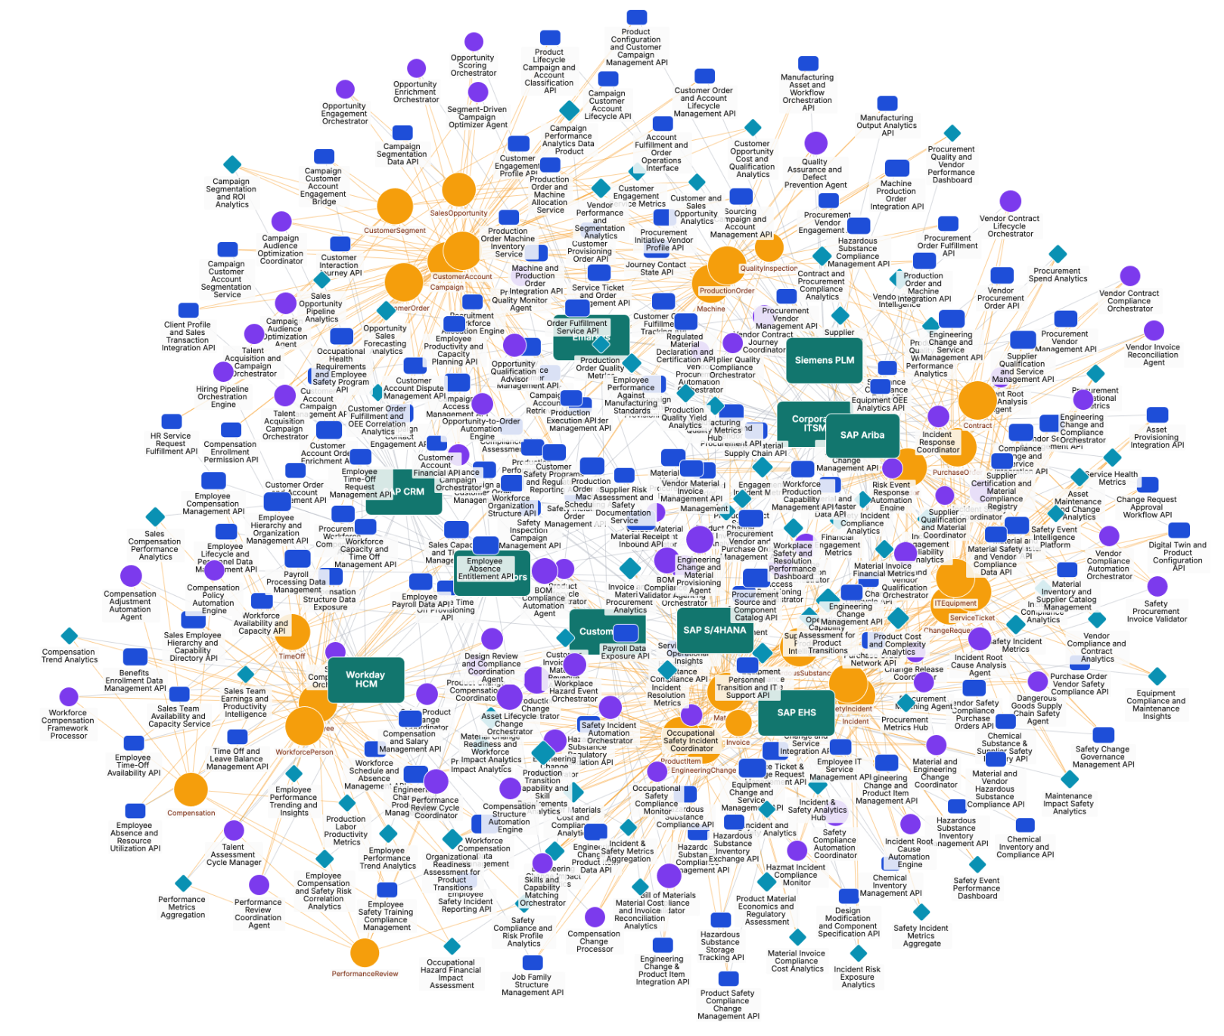
\includegraphics[width=\textwidth]{figures/landscape.png}
  \caption{The 273-resource landscape across 10 systems (green nodes). Resources are typed --- API resources (blue squares), agents (purple circles), data products (diamonds) --- and orange nodes are shared ODM entity types. Edges connect resources through shared entity types, process groups, and process-sequence links. Dense connectivity around shared entity types (e.g.\ \texttt{Material}, \texttt{Compensation}) creates the cross-namespace distractors the ambiguity metric quantifies and the generation pipeline deliberately amplifies.}
  \label{fig:landscape-graph}
\end{figure*}

A design decision behind the ambiguity metric (Appendix~\ref{appendix:landscape}) was to score similarity from ORD fields alone rather than from embeddings, both to keep every tier assignment auditable and to avoid handing embedding-based retrieval a difficulty structure defined in its own representation. To validate this, each of the 273 resources was embedded with \texttt{text-embedding-3-large} using its \texttt{title}, \texttt{shortDescription}, and \texttt{description}, and the embedding cosine of all $\binom{273}{2}=37{,}128$ pairs was compared against the structural ambiguity score. Embeddings were computed after landscape construction and do not influence it. The analysis runs via \path{experiments/embedding_analysis/scripts/embedding_vs_metric.py} and \path{experiments/embedding_analysis/scripts/embedding_by_tier.py}; outputs are in \path{experiments/embedding_analysis/}.

Fig.~\ref{fig:embedding-validation-full}(a) groups all 37{,}128 resource pairs by structural tier and shows a clear monotonic pattern: HIGH-tier pairs reach a median embedding cosine of $0.74$, MEDIUM $0.60$, LOW $0.48$, and unrelated (NONE) $0.35$. What the structural metric marks as confusable is also confusable to an embedding model. Across all pairs, the two similarity scores correlate at $r=0.63$ (Pearson, linear agreement) and $\rho=0.62$ (Spearman, rank agreement), where $1.0$ would mean perfect agreement and $0$ none. A value near $0.63$ means the two measures agree on the overall trend but are not interchangeable. This gap is intentional: the structural metric penalises cross-type pairs and rewards cross-namespace ones, which embedding cosine does not. The benchmark difficulty is therefore not simply a restatement of an embedding retriever's own signal, which keeps the comparison across methods fair.

Projecting the 273 embeddings onto two dimensions with PCA shows two further properties. When coloured by system (Fig.~\ref{fig:embedding-validation-full}(b)), the ten namespaces are fully mixed: resources group by what they do, not by which system they belong to. When coloured by resource type (Fig.~\ref{fig:embedding-validation-full}(c)), a clear split appears, with \texttt{apiResource} in its own region apart from \texttt{agent} and \texttt{dataProduct}. This matches the metric's cross-type penalty. The two shown dimensions capture only about $16\%$ of the total variation, so the real separation is even stronger than the plot suggests.



\definecolor{embHIGH}{HTML}{1C5CAB}
\definecolor{embMED}{HTML}{2A78D6}
\definecolor{embLOW}{HTML}{5598E7}
\definecolor{embNONE}{HTML}{86B6EF}
\definecolor{tpAgent}{HTML}{2A78D6}
\definecolor{tpApi}{HTML}{EB6834}
\definecolor{tpDp}{HTML}{008300}
\definecolor{nsA}{HTML}{2A78D6}
\definecolor{nsB}{HTML}{EB6834}
\definecolor{nsC}{HTML}{008300}
\definecolor{nsD}{HTML}{E34948}
\definecolor{nsE}{HTML}{1BAF7A}
\definecolor{nsF}{HTML}{EDA100}
\definecolor{nsG}{HTML}{4A3AA7}
\definecolor{nsH}{HTML}{E87BA4}
\definecolor{nsI}{HTML}{9D755D}
\definecolor{nsJ}{HTML}{9A9A92}
\begin{figure*}[!t]
  \centering
  \captionsetup[subfigure]{position=top, skip=2pt}
  \begin{subfigure}[t]{0.31\textwidth}
  \centering
  \caption{Cosine by structural tier.}
  \label{fig:emb-tier}
  \begin{tikzpicture}
    \begin{axis}[
      width=\linewidth, height=5.6cm, boxplot/draw direction=y,
      xtick={1,2,3,4}, xticklabels={HIGH\\{\tiny$\geq$0.50}\\{\tiny$n{=}237$}, MEDIUM\\{\tiny .25--.49}\\{\tiny$n{=}1499$}, LOW\\{\tiny .10--.24}\\{\tiny$n{=}6801$}, NONE\\{\tiny$<$.10}\\{\tiny$n{=}28591$}},
      xticklabel style={font=\scriptsize, align=center},
      ymin=0, ymax=1.02, ytick={0,0.2,0.4,0.6,0.8,1.0}, yticklabel style={font=\scriptsize},
      ylabel={Embedding cosine}, ylabel style={font=\scriptsize},
      ymajorgrids, grid style={draw=black!12},
      axis y line*=left, axis x line*=bottom, tick align=outside,
    ]
      \addplot+[boxplot prepared={lower whisker=0.443, lower quartile=0.657, median=0.737, upper quartile=0.811, upper whisker=0.916, draw position=1, box extend=0.5},
        solid, fill=embHIGH, fill opacity=0.9, draw=black!55, line width=0.6pt,
        boxplot/every median/.style={white, line width=1.2pt}] coordinates {};
      \node[font=\tiny\bfseries, white, anchor=south] at (axis cs:1,0.737) {0.74};
      \addplot+[boxplot prepared={lower whisker=0.268, lower quartile=0.500, median=0.599, upper quartile=0.681, upper whisker=0.927, draw position=2, box extend=0.5},
        solid, fill=embMED, fill opacity=0.9, draw=black!55, line width=0.6pt,
        boxplot/every median/.style={white, line width=1.2pt}] coordinates {};
      \node[font=\tiny\bfseries, white, anchor=south] at (axis cs:2,0.599) {0.60};
      \addplot+[boxplot prepared={lower whisker=0.222, lower quartile=0.411, median=0.475, upper quartile=0.538, upper whisker=0.728, draw position=3, box extend=0.5},
        solid, fill=embLOW, fill opacity=0.9, draw=black!55, line width=0.6pt,
        boxplot/every median/.style={white, line width=1.2pt}] coordinates {};
      \node[font=\tiny\bfseries, white, anchor=south] at (axis cs:3,0.475) {0.48};
      \addplot+[boxplot prepared={lower whisker=0.108, lower quartile=0.289, median=0.346, upper quartile=0.410, upper whisker=0.593, draw position=4, box extend=0.5},
        solid, fill=embNONE, fill opacity=0.9, draw=black!55, line width=0.6pt,
        boxplot/every median/.style={white, line width=1.2pt}] coordinates {};
      \node[font=\tiny\bfseries, white, anchor=south] at (axis cs:4,0.346) {0.35};
    \end{axis}
  \end{tikzpicture}
  \end{subfigure}
  \hfill
  \begin{subfigure}[t]{0.31\textwidth}
  \centering
  \caption{By namespace (intermixed).}
  \label{fig:emb-ns}
  \begin{tikzpicture}
    \begin{axis}[
      width=\linewidth, height=5.6cm,
      xmin=-0.6, xmax=0.5, ymin=-0.52, ymax=0.56,
      xtick=\empty, ytick=\empty,
      xlabel={PC1 (9.2\%)}, xlabel style={font=\scriptsize},
      ylabel={PC2 (7.0\%)}, ylabel style={font=\scriptsize},
      axis line style={draw=black!45},
      legend style={at={(0.5,-0.16)}, anchor=north, legend columns=2,
        draw=none, font=\scriptsize, /tikz/every even column/.append style={column sep=3pt}},
      legend image code/.code={\draw[#1,fill=#1] (0.06cm,0) circle (1.6pt);},
    ]
      \addplot[only marks, mark=*, mark size=1.15pt, draw=white, line width=0.15pt, fill=nsA, fill opacity=0.8] coordinates {(0.178,-0.013) (0.233,-0.236) (0.278,0.003) (0.378,-0.116) (0.095,0.383) (0.272,-0.096) (0.213,-0.287) (0.408,0.196) (0.216,0.002) (0.274,-0.229) (0.304,-0.210) (0.266,-0.002) (0.367,0.211) (0.089,0.062) (-0.313,-0.069) (0.104,-0.034) (0.010,-0.061) (-0.306,0.084) (-0.305,0.127) (-0.095,0.147) (-0.089,-0.009) (0.056,-0.172) (-0.308,0.003) (-0.512,0.111) (-0.204,0.093) (-0.292,0.129) (-0.320,0.242) (-0.167,0.192) (-0.235,-0.189)};
      \addlegendentry{\texttt{corp.itsm}}
      \addplot[only marks, mark=*, mark size=1.15pt, draw=white, line width=0.15pt, fill=nsB, fill opacity=0.8] coordinates {(0.168,-0.141) (0.250,-0.195) (-0.000,0.174) (0.141,-0.302) (0.041,0.191) (0.093,-0.319) (0.200,-0.002) (0.238,-0.308) (0.246,-0.303) (0.137,0.295) (0.287,0.193) (0.166,-0.277) (0.344,-0.117) (-0.249,-0.381) (-0.011,0.022) (-0.149,-0.399) (-0.266,-0.046) (-0.036,-0.080) (-0.030,-0.121) (-0.203,-0.298) (-0.175,-0.356) (-0.325,-0.286) (-0.267,-0.054) (-0.275,-0.151) (-0.306,-0.011) (-0.211,-0.044) (-0.506,0.170) (-0.285,-0.250) (-0.247,-0.075)};
      \addlegendentry{\texttt{emarsys.cx}}
      \addplot[only marks, mark=*, mark size=1.15pt, draw=white, line width=0.15pt, fill=nsC, fill opacity=0.8] coordinates {(0.007,-0.098) (0.181,0.120) (0.207,0.058) (0.159,0.305) (0.318,0.214) (0.277,-0.192) (0.207,0.263) (0.256,0.160) (0.295,-0.200) (0.108,0.372) (0.238,-0.271) (0.286,0.075) (0.189,0.043) (0.359,0.278) (0.357,-0.105) (-0.170,0.004) (-0.131,0.220) (0.108,0.026) (0.012,0.292) (-0.272,0.335) (-0.194,0.046) (-0.281,-0.137) (-0.263,0.124) (-0.496,0.129) (-0.229,0.031) (-0.162,-0.156) (-0.224,0.194) (-0.422,-0.063) (-0.224,0.104)};
      \addlegendentry{\texttt{my.mes}}
      \addplot[only marks, mark=*, mark size=1.15pt, draw=white, line width=0.15pt, fill=nsD, fill opacity=0.8] coordinates {(0.358,0.132) (0.291,-0.113) (0.223,-0.114) (0.280,0.164) (0.377,0.094) (0.398,0.311) (0.286,0.177) (0.314,0.336) (0.303,0.325) (0.203,0.150) (0.329,0.005) (0.142,0.462) (0.351,0.326) (-0.100,0.081) (-0.173,0.288) (-0.042,0.085) (-0.264,0.115) (-0.215,0.321) (-0.255,-0.092) (-0.162,0.217) (-0.276,-0.005) (-0.246,0.176) (-0.302,0.214)};
      \addlegendentry{\texttt{sap.ariba}}
      \addplot[only marks, mark=*, mark size=1.15pt, draw=white, line width=0.15pt, fill=nsE, fill opacity=0.8] coordinates {(0.242,-0.052) (0.107,-0.287) (0.314,-0.026) (0.019,-0.354) (0.011,-0.348) (0.218,-0.310) (0.323,-0.129) (0.243,-0.251) (0.343,-0.007) (0.180,-0.057) (0.392,0.198) (-0.193,-0.248) (-0.153,-0.081) (-0.012,0.085) (-0.198,-0.307) (-0.213,-0.432) (-0.215,-0.413) (-0.150,-0.190) (-0.285,-0.218) (-0.392,0.036) (-0.210,-0.008) (-0.359,-0.275) (-0.019,0.258) (-0.315,-0.296) (-0.323,-0.275) (-0.290,-0.021) (-0.091,-0.004)};
      \addlegendentry{\texttt{sap.crm}}
      \addplot[only marks, mark=*, mark size=1.15pt, draw=white, line width=0.15pt, fill=nsF, fill opacity=0.8] coordinates {(0.113,0.334) (0.297,0.289) (0.004,0.397) (0.097,-0.040) (0.062,0.367) (0.108,0.267) (0.105,0.313) (-0.109,0.096) (0.025,0.055) (0.078,0.187) (0.109,0.255) (0.097,0.468) (0.153,0.380) (0.094,0.099) (0.095,0.165) (-0.363,-0.002) (-0.105,0.257) (-0.293,0.001) (-0.138,0.308) (-0.203,-0.163) (-0.118,0.194) (-0.467,0.116) (-0.339,0.168) (-0.288,0.396) (-0.329,-0.001) (-0.440,0.131) (-0.294,0.367) (-0.430,0.057) (-0.391,0.093) (-0.296,0.007)};
      \addlegendentry{\texttt{sap.ehs}}
      \addplot[only marks, mark=*, mark size=1.15pt, draw=white, line width=0.15pt, fill=nsG, fill opacity=0.8] coordinates {(0.230,0.242) (0.157,-0.100) (0.243,-0.199) (0.175,0.179) (0.380,-0.091) (0.276,-0.120) (0.108,0.343) (0.284,-0.077) (0.233,-0.126) (0.245,0.123) (0.144,0.342) (-0.017,0.147) (0.228,-0.269) (0.371,-0.088) (-0.050,0.111) (0.026,0.243) (0.070,-0.006) (-0.036,-0.216) (-0.328,0.016) (-0.022,-0.013) (-0.188,0.185) (-0.111,0.258) (-0.298,0.181) (-0.224,0.098) (-0.251,0.014) (-0.325,0.173) (-0.248,0.030) (-0.011,-0.086)};
      \addlegendentry{\texttt{sap.s4}}
      \addplot[only marks, mark=*, mark size=1.15pt, draw=white, line width=0.15pt, fill=nsH, fill opacity=0.8] coordinates {(0.176,-0.177) (0.152,-0.190) (0.075,-0.282) (0.224,-0.215) (0.257,-0.206) (0.241,-0.247) (0.367,0.152) (0.164,-0.192) (0.235,-0.076) (0.293,-0.194) (0.235,0.066) (0.268,-0.151) (0.168,0.145) (0.071,-0.242) (-0.018,-0.002) (-0.178,-0.262) (-0.158,-0.282) (-0.126,-0.387) (-0.037,-0.187) (-0.126,-0.398) (-0.320,0.144) (-0.355,-0.252) (-0.374,0.064) (-0.183,-0.081) (-0.071,-0.062) (-0.261,-0.257)};
      \addlegendentry{\texttt{sap.sf}}
      \addplot[only marks, mark=*, mark size=1.15pt, draw=white, line width=0.15pt, fill=nsI, fill opacity=0.8] coordinates {(0.256,0.065) (0.211,0.211) (0.071,-0.030) (0.180,-0.015) (0.336,0.002) (0.217,0.076) (0.190,-0.245) (0.230,-0.014) (0.289,-0.101) (-0.007,0.395) (0.126,-0.204) (0.158,0.350) (0.089,0.352) (0.112,-0.166) (-0.011,0.256) (0.099,0.087) (-0.207,0.007) (-0.058,0.262) (-0.118,0.050) (-0.020,0.263) (-0.204,-0.002) (-0.018,0.077) (-0.083,0.141) (-0.352,0.176) (-0.248,-0.084) (-0.241,0.196)};
      \addlegendentry{\texttt{siemens.plm}}
      \addplot[only marks, mark=*, mark size=1.15pt, draw=white, line width=0.15pt, fill=nsJ, fill opacity=0.8] coordinates {(0.219,-0.246) (0.228,-0.164) (0.144,-0.213) (0.263,-0.126) (0.266,-0.184) (0.060,-0.137) (0.236,-0.270) (0.215,-0.184) (0.321,-0.223) (0.285,-0.109) (-0.125,0.391) (0.077,-0.121) (0.177,-0.238) (-0.199,-0.300) (-0.147,0.058) (-0.165,-0.250) (-0.126,-0.244) (-0.138,-0.180) (-0.154,-0.211) (-0.281,0.080) (-0.110,-0.246) (-0.102,-0.253) (-0.376,-0.248) (-0.340,-0.232) (-0.451,0.087) (-0.041,-0.039)};
      \addlegendentry{\texttt{workday.hcm}}
    \end{axis}
  \end{tikzpicture}
  \end{subfigure}
  \hfill
  \begin{subfigure}[t]{0.31\textwidth}
  \centering
  \caption{By resource type (separated).}
  \label{fig:emb-type}
  \begin{tikzpicture}
    \begin{axis}[
      width=\linewidth, height=5.6cm,
      xmin=-0.6, xmax=0.5, ymin=-0.52, ymax=0.56,
      xtick=\empty, ytick=\empty,
      xlabel={PC1 (9.2\%)}, xlabel style={font=\scriptsize},
      ylabel={PC2 (7.0\%)}, ylabel style={font=\scriptsize},
      axis line style={draw=black!45},
      legend style={at={(0.5,-0.16)}, anchor=north, legend columns=1,
        draw=none, font=\scriptsize, /tikz/every even column/.append style={column sep=3pt}},
      legend image code/.code={\draw[#1,fill=#1] (0.06cm,0) circle (1.6pt);},
    ]
      \addplot[only marks, mark=*, mark size=1.15pt, draw=white, line width=0.15pt, fill=tpAgent, fill opacity=0.8] coordinates {(-0.313,-0.069) (0.104,-0.034) (0.010,-0.061) (-0.306,0.084) (-0.305,0.127) (-0.095,0.147) (-0.089,-0.009) (0.056,-0.172) (-0.249,-0.381) (-0.011,0.022) (-0.149,-0.399) (-0.266,-0.046) (-0.036,-0.080) (-0.030,-0.121) (-0.203,-0.298) (-0.175,-0.356) (-0.170,0.004) (-0.131,0.220) (0.108,0.026) (0.012,0.292) (-0.272,0.335) (-0.100,0.081) (-0.173,0.288) (-0.042,0.085) (-0.193,-0.248) (-0.153,-0.081) (-0.012,0.085) (-0.198,-0.307) (-0.213,-0.432) (-0.215,-0.413) (-0.150,-0.190) (-0.363,-0.002) (-0.105,0.257) (-0.293,0.001) (-0.138,0.308) (-0.203,-0.163) (-0.118,0.194) (-0.050,0.111) (0.026,0.243) (0.070,-0.006) (-0.036,-0.216) (-0.328,0.016) (-0.022,-0.013) (-0.178,-0.262) (-0.158,-0.282) (-0.126,-0.387) (-0.037,-0.187) (-0.126,-0.398) (-0.320,0.144) (-0.011,0.256) (0.099,0.087) (-0.207,0.007) (-0.058,0.262) (-0.118,0.050) (-0.020,0.263) (-0.204,-0.002) (-0.018,0.077) (-0.199,-0.300) (-0.147,0.058) (-0.165,-0.250) (-0.126,-0.244) (-0.138,-0.180) (-0.154,-0.211) (-0.281,0.080) (-0.110,-0.246) (-0.102,-0.253)};
      \addlegendentry{\texttt{agent}}
      \addplot[only marks, mark=*, mark size=1.15pt, draw=white, line width=0.15pt, fill=tpApi, fill opacity=0.8] coordinates {(0.178,-0.013) (0.233,-0.236) (0.278,0.003) (0.378,-0.116) (0.095,0.383) (0.272,-0.096) (0.213,-0.287) (0.408,0.196) (0.216,0.002) (0.274,-0.229) (0.304,-0.210) (0.266,-0.002) (0.367,0.211) (0.089,0.062) (0.168,-0.141) (0.250,-0.195) (-0.000,0.174) (0.141,-0.302) (0.041,0.191) (0.093,-0.319) (0.200,-0.002) (0.238,-0.308) (0.246,-0.303) (0.137,0.295) (0.287,0.193) (0.166,-0.277) (0.344,-0.117) (0.007,-0.098) (0.181,0.120) (0.207,0.058) (0.159,0.305) (0.318,0.214) (0.277,-0.192) (0.207,0.263) (0.256,0.160) (0.295,-0.200) (0.108,0.372) (0.238,-0.271) (0.286,0.075) (0.189,0.043) (0.359,0.278) (0.357,-0.105) (0.358,0.132) (0.291,-0.113) (0.223,-0.114) (0.280,0.164) (0.377,0.094) (0.398,0.311) (0.286,0.177) (0.314,0.336) (0.303,0.325) (0.203,0.150) (0.329,0.005) (0.142,0.462) (0.351,0.326) (0.242,-0.052) (0.107,-0.287) (0.314,-0.026) (0.019,-0.354) (0.011,-0.348) (0.218,-0.310) (0.323,-0.129) (0.243,-0.251) (0.343,-0.007) (0.180,-0.057) (0.392,0.198) (0.113,0.334) (0.297,0.289) (0.004,0.397) (0.097,-0.040) (0.062,0.367) (0.108,0.267) (0.105,0.313) (-0.109,0.096) (0.025,0.055) (0.078,0.187) (0.109,0.255) (0.097,0.468) (0.153,0.380) (0.094,0.099) (0.095,0.165) (0.230,0.242) (0.157,-0.100) (0.243,-0.199) (0.175,0.179) (0.380,-0.091) (0.276,-0.120) (0.108,0.343) (0.284,-0.077) (0.233,-0.126) (0.245,0.123) (0.144,0.342) (-0.017,0.147) (0.228,-0.269) (0.371,-0.088) (0.176,-0.177) (0.152,-0.190) (0.075,-0.282) (0.224,-0.215) (0.257,-0.206) (0.241,-0.247) (0.367,0.152) (0.164,-0.192) (0.235,-0.076) (0.293,-0.194) (0.235,0.066) (0.268,-0.151) (0.168,0.145) (0.071,-0.242) (-0.018,-0.002) (0.256,0.065) (0.211,0.211) (0.071,-0.030) (0.180,-0.015) (0.336,0.002) (0.217,0.076) (0.190,-0.245) (0.230,-0.014) (0.289,-0.101) (-0.007,0.395) (0.126,-0.204) (0.158,0.350) (0.089,0.352) (0.112,-0.166) (0.219,-0.246) (0.228,-0.164) (0.144,-0.213) (0.263,-0.126) (0.266,-0.184) (0.060,-0.137) (0.236,-0.270) (0.215,-0.184) (0.321,-0.223) (0.285,-0.109) (-0.125,0.391) (0.077,-0.121) (0.177,-0.238)};
      \addlegendentry{\texttt{apiResource}}
      \addplot[only marks, mark=*, mark size=1.15pt, draw=white, line width=0.15pt, fill=tpDp, fill opacity=0.8] coordinates {(-0.308,0.003) (-0.512,0.111) (-0.204,0.093) (-0.292,0.129) (-0.320,0.242) (-0.167,0.192) (-0.235,-0.189) (-0.325,-0.286) (-0.267,-0.054) (-0.275,-0.151) (-0.306,-0.011) (-0.211,-0.044) (-0.506,0.170) (-0.285,-0.250) (-0.247,-0.075) (-0.194,0.046) (-0.281,-0.137) (-0.263,0.124) (-0.496,0.129) (-0.229,0.031) (-0.162,-0.156) (-0.224,0.194) (-0.422,-0.063) (-0.224,0.104) (-0.264,0.115) (-0.215,0.321) (-0.255,-0.092) (-0.162,0.217) (-0.276,-0.005) (-0.246,0.176) (-0.302,0.214) (-0.285,-0.218) (-0.392,0.036) (-0.210,-0.008) (-0.359,-0.275) (-0.019,0.258) (-0.315,-0.296) (-0.323,-0.275) (-0.290,-0.021) (-0.091,-0.004) (-0.467,0.116) (-0.339,0.168) (-0.288,0.396) (-0.329,-0.001) (-0.440,0.131) (-0.294,0.367) (-0.430,0.057) (-0.391,0.093) (-0.296,0.007) (-0.188,0.185) (-0.111,0.258) (-0.298,0.181) (-0.224,0.098) (-0.251,0.014) (-0.325,0.173) (-0.248,0.030) (-0.011,-0.086) (-0.355,-0.252) (-0.374,0.064) (-0.183,-0.081) (-0.071,-0.062) (-0.261,-0.257) (-0.083,0.141) (-0.352,0.176) (-0.248,-0.084) (-0.241,0.196) (-0.376,-0.248) (-0.340,-0.232) (-0.451,0.087) (-0.041,-0.039)};
      \addlegendentry{\texttt{dataProduct}}
    \end{axis}
  \end{tikzpicture}
  \end{subfigure}
  \caption{Post-hoc embedding validation on the 273-resource landscape. \textbf{(a)}~Embedding cosine rises monotonically with the structural ambiguity tier (median 0.74 / 0.60 / 0.48 / 0.35 for HIGH/MEDIUM/LOW/NONE): pairs the field-based metric marks as confusable are independently confusable to an embedding model. \textbf{(b)}~In PCA-projected embedding space the ten namespaces are thoroughly intermixed, with no system forming its own cluster. Resources from different systems sit close together when they serve the same business function. \textbf{(c)}~Resource types form distinct regions, consistent with the metric's cross-type penalty. PC1$+$PC2 capture only 16\% of variance (embeddings are 3072-dimensional), so the projection understates the separation.}
  \label{fig:embedding-validation-full}\end{figure*}


% ─────────────────────────────────────────────────────────────────────────────

\subsection{Disambiguation Analysis}
\label{appendix:disambiguation}
% ─────────────────────────────────────────────────────────────────────────────

This appendix details how the semantic enrichment fields affect pairwise resource ambiguity and how that effect compares to embedding similarity. On the clean landscape, structural ambiguity metric and cosine similarity broadly agree ($r=0.63$, App.~\ref{appendix:landscape-results}, Fig.~\ref{fig:embedding-validation-full}). To evaluate whether enrichment reduces ambiguity between confusable resource pairs, the base metric is extended with the three semantic fields. The analysis in Sec.~\ref{sec:results} argues that ambiguity is a property of the representation, not of the resources; the results here confirm this: structural ambiguity falls while embedding cosine rises on the same pairs.

\textbf{Extended ambiguity metric.} The benchmark's ambiguity metric (Sec.~\ref{sec:design}, App.~\ref{appendix:landscape}) scores each resource pair over six ORD fields (\texttt{text}, \texttt{localId}, \texttt{entityTypes}, \texttt{lineOfBusiness}, \texttt{tags}, \texttt{industry}). For this analysis it is extended with three design-time semantic fields: \texttt{capabilities} and \texttt{partOfGroups} scored by Jaccard overlap, and \texttt{useCases} scored by TF-IDF cosine. The field \texttt{processNext} is excluded because it encodes directed process ordering between resources rather than a property of a single resource. A semantic field enters the score only when both resources in a pair carry it, so the denominator grows from 6 to at most 9. This ensures a score can only fall when two resources actively describe different capabilities or use cases, not as an artefact of a larger denominator. Tab.~\ref{tab:extended-metric} lists all nine dimensions.

\begin{table*}[!t]
  \renewcommand{\arraystretch}{1.2}
  \caption{Extended ambiguity metric: nine dimensions with scoring method, an excerpt of the actual field contents of each resource, and the resulting sub-score for the \texttt{AssetProvisioningOrchestrator} (A, \texttt{corp.itsm}) vs \texttt{AssetLifecycleChangeOrchestrator} (B, \texttt{sap.s4}) pair. Identical \texttt{tags} give 1.00, but the disjoint \texttt{capabilities} and \texttt{partOfGroups} give 0.00. The three semantic fields are added only when both resources carry them; the denominator grows from 6 to 9 only for those active dimensions. Structural ambiguity therefore falls from 0.75 to 0.53, while embedding cosine rises from 0.79 to 0.82.}
  \label{tab:extended-metric}
  \centering\scriptsize
  \begin{tabularx}{\textwidth}{@{} l l X X r @{}}
  \toprule
  \textbf{Dimension} & \textbf{Scoring} & \textbf{Resource A (excerpt)} & \textbf{Resource B (excerpt)} & \textbf{Score} \\
  \midrule
  \multicolumn{5}{@{}l}{\textit{Original six fields}} \\
  \texttt{text}            & TF-IDF cosine, title+desc & ``Asset Provisioning Orchestrator'' & ``Asset Lifecycle Change Orchestrator'' & 0.60 \\
  \texttt{localId}         & Jaccard, CamelCase tokens & AssetProvisioning\-Orchestrator & AssetLifecycleChange\-Orchestrator & 0.40 \\
  \texttt{entityTypes}     & IDF-weighted Jaccard & (none) & (none) & 1.00 \\
  \texttt{lineOfBusiness}  & Jaccard & it-service-management & it-service-management & 1.00 \\
  \texttt{tags}            & Jaccard & asset-lifecycle, change-automation, provisioning-orchestration & asset-lifecycle, change-automation, provisioning-orchestration & 1.00 \\
  \texttt{industry}        & Jaccard & (none) & (none) & 0.00 \\
  \multicolumn{5}{@{}l}{\textit{Semantic extension}} \\
  \texttt{capabilities}    & Jaccard, verb-noun tokens & orchestrate-asset-provisioning, allocate-materials, \ldots & orchestrate-engineering-change, manage-change-approvals, \ldots & 0.00 \\
  \texttt{partOfGroups}    & Jaccard, group IDs & ProductTransitionSafety\-Coordination, \ldots & product\_launch\_qa, ChangeTalentIntegration & 0.00 \\
  \texttt{useCases}        & TF-IDF cosine & ``provisions change-related equipment to production floor'' & ``coordinate approvals from manufacturing, supply chain, HR'' & 0.29 \\
  \midrule
  Cross-ns bonus & $+0.5$ cross-namespace & \multicolumn{2}{l}{\texttt{corp.itsm} vs \texttt{sap.s4} (cross-namespace)} & $+0.5$ \\
  Type penalty & $\times 0.5$ if types differ & \multicolumn{2}{l}{both \texttt{agent} (same type)} & $\times 1.0$ \\
  \midrule
  \multicolumn{4}{@{}l}{\textbf{Formula:} $\text{sim}^+(a,b) = (\sum_{d \in D \cup D^+_{ab}} s_d + 0.5_{\text{cross-ns}}) / (6 + |D^+_{ab}|)$} & \\
  \multicolumn{4}{@{}l}{\phantom{\textbf{Formula:} }\textbf{Structural ambiguity:}\ Clean $(|D|{=}6)$ \textbf{0.75} $\rightarrow$ Enriched $(|D|{=}9)$ \textbf{0.53}} & \\
  \multicolumn{4}{@{}l}{\phantom{\textbf{Formula:} }\textbf{Embedding cosine} (\texttt{text-embedding-3-large}):\ Clean \textbf{0.79} $\rightarrow$ Enriched \textbf{0.82}} & \\
  \bottomrule
  \end{tabularx}
\end{table*}

Tab.~\ref{tab:extended-metric} applies the extended metric to one HIGH-tier pair. \texttt{AssetProvisioningOrchestrator} and \texttt{AssetLifecycleChangeOrchestrator} share entity types, line of business, tags, and text, giving a clean structural score of 0.75. Their capabilities and process groups are disjoint, so adding semantic fields lowers the score to 0.53. The embedding moves in the opposite direction: cosine rises from 0.79 to 0.82 because the added text increases token overlap.

\textbf{Populations and mean ambiguity.} The analysis runs on the 70 resources that carry all semantic fields, giving 2\,415 unordered pairs where both sides are enriched and the extended metric can act on both. Fig.~\ref{fig:disambiguation} reports the mean pairwise ambiguity under the original versus the extended metric for two groups: all 2\,415 enriched pairs (0.111~$\rightarrow$~0.084, $-24.5\%$) and the 85 of them that were HIGH-tier (sim~$\geq$~0.50) under the original metric (0.643~$\rightarrow$~0.461, $-28.3\%$). The HIGH-tier subset isolates the pairs that actually risk confusion and shows the larger relative drop: semantic enrichment reduces structural ambiguity most where it matters.

\textbf{Embedding contrast on the same pairs.} Embedding cosine moves opposite to the structural drop. Embeddings are computed with \texttt{text-embedding-3-large}. The clean text concatenates \texttt{title}, \texttt{shortDescription}, and \texttt{description}, while the enriched text appends \texttt{partOfGroups}, \texttt{processNext}, \texttt{capabilities}, and \texttt{useCases} separated by the \texttt{|} character. Fig.~\ref{fig:disambiguation-embedding} reports cosine for three pair types. For all 2\,415 both-enriched pairs the mean cosine \emph{rises} from 0.392 to 0.501 ($+27.7\%$). For the 85 previously HIGH-tier pairs it rises from 0.720 to 0.761 ($+5.7\%$). For the 14\,210 mixed pairs where only one resource is enriched it rises from 0.368 to 0.388 ($+5.3\%$). The mixed case is the clearest one. The structural ambiguity metric leaves such a pair unchanged because the semantic dimensions need both sides, yet enriching one resource alone shifts its vector toward the shared topical region and raises cosine.


\textbf{The two directions are not a contradiction.} A metric that lowers ambiguity and an embedding that raises similarity on the same pairs look contradictory at first, but they are not. Ambiguity is not an absolute property of two resources; it is a property of how a retrieval method represents them, and the two representations genuinely disagree about whether these pairs are easy to tell apart. They move in opposite directions for the same underlying reason. The structural metric compares each semantic field on its own, so two resources with disjoint capability sets score zero on that dimension and are pushed apart. The embedding instead compresses every field into one vector, so appending more topically related text moves both vectors toward the same region and raises cosine similarity in all three pair types above, including mixed pairs where only one resource gains fields. Enrichment therefore lowers ambiguity only for methods that read the typed fields as discrete signals (namespace, entity-type membership, graph edges, capability filters); a method that retrieves purely by embedding distance sees the opposite effect. This structural alignment between retrieval mechanism and enriched field type is the central qualification on the assumption that richer descriptions uniformly improve selection. The full computation is implemented in \texttt{experiments/disambiguation/}.


\end{document}
